\documentclass{beamer}
\usepackage[utf8]{inputenc}
\usepackage{hyperref}

\usepackage{tikz}

\usepackage{latexsym,xcolor,multicol,booktabs,calligra}
\usepackage{amsmath,amssymb,BOONDOX-cal,bm}	
\usepackage{graphicx,pstricks,stackengine} 
\usepackage{libertinus}
\usepackage{amssymb}
\usepackage{pgfplots}
\usepackage{tikz}
\usepackage{xcolor}
\usetikzlibrary{positioning}

\usepackage{etoolbox}
\makeatletter
\newcommand{\noframenumbering}{%
  \beamer@noframenumberingtrue%
}
\makeatother






\usepackage[T1]{fontenc}

\title{Macroeconometrics\\
5 - Structural VAR, Identification, and Policy Shock Assessment}
\author{Camille Souffron\\
Ecole Normale Supérieure \& Paris School of Economics\\
\textcolor{blue}{\href{mailto:camille.souffron@ens.psl.eu}{camille.souffron@ens.psl.eu}}}
\institute{\normalsize M2 EPOG JM}
\date{Fall 2026}

\usetheme{Singapore}

\def\cmd#1{\texttt{\color{red}\footnotesize $\backslash$#1}}
\def\env#1{\texttt{\color{RoyalBlue}\footnotesize #1}}

\newtheorem{thm}{Theorem}[theorem]
\setbeamertemplate{footline}[frame number]




\begin{document}



\begin{frame} % <-- no [plain] here!
    \titlepage % This keeps the theme style
    \begin{center}
        
\includegraphics[width=0.5\textwidth]{logos.png}
    \end{center}
\end{frame}



\addtocounter{framenumber}{-1}

% Roadmap
\begin{frame}{Course Roadmap}
\small
\begin{enumerate}
  \item \textbf{Introduction to Time Series Analysis 1/2}  

  \item   \textbf{Introduction to Time Series Analysis 2/2}

  \item \textbf{AR, MA, ARMA Processes and Forecast}  

  \item \textbf{VAR Models}  

  \item \textbf{Structural VARs, Identification and Policy Impact:}  
  Short- and long-run restrictions, sign restrictions, narrative approach.

  \item \textbf{Nonlinear Models:}  
  Threshold, Smooth Transition, Markov-Switching Regimes, Local Projections (LP), Time-Varying Parameters

  \item \textbf{Cointegration (VECM) \& Dynamic Factor Models (DFM)}  

  \item \textbf{Calibration \& Estimation of Structural Models I:}  
  (Over/Under)Identification, Empirical SFC \& IO.

  \item \textbf{Calibration \& Estimation of Structural Models II:} GMM, SMM.

  \item \textbf{Calibration \& Estimation of Structural Models III:}  
  Model resolution, Agent-Based Models (ABM).
  \begin{enumerate}
      \item If time: \textbf{Bibliometrics, Meta-Analysis (\& Spectral Methods)}
  \end{enumerate}
\end{enumerate}
\end{frame}



%======================================================
\begin{frame}{NB: how far can we forecast with ARIMA / VAR?}
%======================================================

\small

 \textbf{With horizon growing, forecast uncertainty explodes}, forecast point converges to the unconditional mean (linear models), and economic content vanishes quickly (forecast variance grows, mostly noise). 

\medskip

\begin{itemize}\itemsep4pt
    \item \textbf{ARIMA (quarterly):} reliable for \textbf{1-8 quarters (2y)}, fragile beyond.
    \item \textbf{Small VAR (2-4 vars):} meaningful up to \textbf{8-12 quarters (2-3y)}.
    \item \textbf{Large VARs:} shorter horizon due to parameter uncertainty, except if Bayesian dimension regularisation.
    \item Then anyway, since \textit{\textbf{linear and stable (stationary)}} model: converges back to mean ($0$ if $\mu=0$)
\end{itemize}

\medskip

\textbf{In practice:}
\begin{itemize}\itemsep4pt
    \item Central banks (Fed/ECB) rarely forecast beyond \textbf{8-12 quarters}.
    \item Academic VAR papers: IRFs often shown to \textbf{16-20 quarters}, but forecasts trusted only \textbf{1-3 years} (since other events will accumulate).
\end{itemize}

\end{frame}

\section{Causality?}

\begin{frame}{But what about \textit{\textbf{causality?}}}
So far: only \textit{\textbf{reduced-form}} VAR.
\medskip

Whereas the VAR model is able to capture efficiently the interactions between the different variables, it does not allow to reveal the underlying causal mechanisms since two different causal schemes can correspond to the same reduced forms: \textbf{\textit{observational equivalence.}}
\medskip

Innovation $u_{t,k}$ on variable $y_{t,k}$ i.e. linearly unpredictable:\textbf{ no reason \textit{a priori} to be orthogonal} to the other variables (i.e. to be a "structural" shock")! Can be\textbf{a contemporaneous feedback from other variables!} Or can be the fruit of a \textbf{common shock on the whole system}!
\medskip

E.g. assessing the impact (IRF) of a monetary policy: an increase in interest rates in response to economic conditions is NOT considered as a shock, it is endogenous! Same for FEVD.
\end{frame}



\begin{frame}{A trivial example}
\textbf{Public policies are state-dependent}

\begin{itemize}
  \item \textbf{Monetary policy reacts to the state of the economy}: inflation, output, unemployment, credit spreads, exchange rates, asset prices, forecasts, financial stability assessments, etc.
  \item \textbf{Naïve idea:} hence, if we simply look at "what happened after" a policy move, we confound \textbf{policy shock} (actually the systematic reaction to $(\pi_t, y_t, unemp_t...)$) and the evolution of the \textbf{current conjuncture}!
  \item Any better idea?
\pause
\item Why not estimate a Taylor rule (for the systematic policy response by the Central Bank), and take the \textbf{residual} $u_t$ as the policy shock that can't be explain by the systematic policy rule? 
\textbf{\item Actually: NO, because of contemporaneity}

\end{itemize}
\end{frame}



%======================================================
\begin{frame}{Causal mechanisms in a stylized economy}
%======================================================
\small
\begin{itemize}
    \item Let’s start from the \textbf{structural (theoretical) side}.
    \item Suppose our macroeconomy is summarized by three key variables:
          output growth $g_t$, nominal interest rate $i_t$, and inflation $\pi_t$.
          \begin{itemize}
              \item $g_t$ reacts to real shocks $\varepsilon_{r,t}$,
        \item $\pi_t$ reacts to cost-push shocks $\varepsilon_{n,t}$,
        \item $i_t$ follows a Taylor rule and reacts to monetary-policy shocks $\varepsilon_{mp,t}$.
\end{itemize}

    \item We posit \textbf{causal equations} linking them, inspired by
          standard semi-structural relationships (IS curve, Taylor rule, Phillips curve).
\end{itemize}
\end{frame}

%======================================================
\begin{frame}{The structural system (true DGP)}
%======================================================

\[
B_0y_t = B_1 y_{t-1} + \varepsilon_t, \qquad \varepsilon_t \sim \mathcal{N}(0,I_k),
\qquad u_t =  B_0^{-1}\,\varepsilon_t.
\]
With $B_0=$ contemporaneous relationships matrix.
\[
\left\{
\begin{aligned}
g_t &= -0.3(i_{t-1} - \pi_{t-1}) + \varepsilon_{r,t} &\quad &\text{(IS curve)}\\[4pt]
i_t &= 0.9 i_{t-1} + 1.5 \pi_t + \varepsilon_{mp,t} &\quad &\text{(Taylor rule)}\\[4pt]
\pi_t &= 0.9 \pi_{t-1} + 0.2 g_{t-1} + \varepsilon_{n,t} &\quad &\text{(Backward-looking Phillips curve)}
\end{aligned}
\right.
\]
\begin{itemize}
  \item $\varepsilon_{r,t}, \varepsilon_{mp,t}, \varepsilon_{n,t}$ are uncorrelated \textbf{structural "shocks"}, \textbf{mutually uncorrelated.}
  \item They represent the \textbf{true causal innovations} driving the economy.
\end{itemize}
\end{frame}



%======================================================
\begin{frame}{From structural to reduced form}
%======================================================

\begin{itemize}
  \item To express the model in VAR form, eliminate contemporaneous $\pi_t$ from RHS, by developping it:\footnote{\footnotesize Btw: you cannot estimate the structural form by OLS because the contemporaneous regressors are jointly determined with the structural shocks, so they are correlated with the equation’s error term (thus violating the fundamental OLS exogeneity condition). }
\[
\begin{aligned}
g_t &= 0.06 g_{t-1} - 0.3 i_{t-1} + 0.27 \pi_{t-1} + 0.3\varepsilon_{n,t} + \varepsilon_{r,t},\\
i_t &= 0.9 i_{t-1} + 1.35 \pi_{t-1} + 0.3 g_{t-1} + \varepsilon_{mp,t} + 1.5\varepsilon_{n,t},\\
\pi_t &= 0.9 \pi_{t-1} + 0.2 g_{t-1} + \varepsilon_{n,t}.
\end{aligned}
\]
  \item Now all RHS variables are \textbf{lagged} - this is the \textbf{reduced form VAR}.
  \item But note: shocks $\varepsilon_t$ appear mixed in the residuals.
\end{itemize}
\end{frame}


\subsection{}

%======================================================
\begin{frame}{Why a reduced-form VAR cannot identify causality}
%======================================================

\textbf{So the reduced form we actually estimate is} (with $A= B_0^{-1} B_1$):
\[
y_t = A y_{t-1} + u_t, \qquad u_t \sim \mathcal{N}(0,\Sigma_u),
\qquad u_t = B_0^{-1}\,\varepsilon_t.
\]

Because the central bank reacts to inflation \emph{within the period} (Taylor rule), \textbf{the reduced-form innovations $u_t$ \emph{mix} structural shocks (through $B_0^{-1}$ the impact matrix, i.e. the inverse of the matrix of contemporaneous relations $B_0$)}
\bigskip

\textbf{Look at the interest-rate "innovation":}
\[
\boxed{
u_{i,t} = \varepsilon_{mp,t} \;+\; 1.5\,\varepsilon_{n,t}
}
\]
Reduced-form innovations $u_t$ are\textbf{ \emph{correlated}:} $\Sigma_u$ generally \textbf{non-diagonal,} and same reduced form $(A,\Sigma_u)$ admits\textbf{ infinitely many} $B_0$, each delivering \emph{different} "structural" shocks/IRFs and $\Sigma_\varepsilon \text{ diagonal}$ (identification problem).  

\end{frame}




%======================================================
\begin{frame}{Why "regress \& take residual" is not enough}
%======================================================

So we \textbf{CAN'T} estimate a backward-looking Taylor rule and take the residual as the monetary policy shock (i.e. the non-systematic policy response): 
\[
i_t = r^* + \phi_\pi \pi_t + \phi_y y_t + u_t
\quad\Rightarrow\quad
\text{"shock" } = u_t
\]
\begin{itemize}
  \item If $i_t$ itself react \emph{within the period} to $y_t,\pi_t$, thus to other shocks ($\varepsilon^y_t,\varepsilon^\pi_t$): the
\textbf{contemporaneous} part remains in the residual.

\medskip
\item The single-equation residual $u_t$ is \emph{not} an isolated monetary policy shock but a linear combination of several structural shocks. 
\item We thus need a \textbf{structural VAR} (restrictions on $ B_0^{-1}$). 
\item (And we'll see later that CB uses a larger information set, justifying the \textit{narrative approach}).
\end{itemize}
\end{frame}



\begin{frame}{Why $\Sigma_u$ Is not enough}

You observe only how the shocks \emph{co-move}, not what \emph{generated} them.

\medskip
$\Sigma_u$ tells you:
\begin{itemize}
    \item ``shock 1 and shock 2 are correlated by $0.3$'',
    \item ``shock 1 has variance $0.7$''.
\end{itemize}

\medskip
But that correlation could arise:
\begin{itemize}
    \item because \textbf{structural shock A} affects both variables,
    \item or because \textbf{structural shock B} hits variable 1 first,
    \item or because both respond to a \textbf{common shock},
    \item or because the \textbf{matrix of contemporaneous relations }$B_0$ mixes them.
\end{itemize}

\end{frame}


%======================================================
\begin{frame}{Why a reduced-form VAR cannot identify causality}
%======================================================
\textbf{Interpretation (very important):}
\begin{itemize}
    \item The VAR sees only $u_{i,t}$.
    \item But $u_{i,t}$ is \emph{not} a monetary policy shock.
    \item It contains:
    \begin{itemize}
        \item a true policy shock: $\varepsilon_{mp,t}$,
        \item \emph{plus} a contemporaneous inflation (cost-push) shock: $1.5\,\varepsilon_{n,t}$.
    \end{itemize}
    \item Therefore: IRFs to $u_{i,t}$ \textbf{do not give} the causal effect of monetary policy.
\end{itemize}
\medskip
\[
\text{Reduced-form VAR shocks} \neq \text{structural economic shocks}.
\]
\[
\text{Reduced-form VAR} \Rightarrow \text{prediction, not causality}.
\]
To obtain causal IRFs and FEVD, we must \emph{identify} the structural shocks (Cholesky decomposition, assuming structural relationships (theory), sign restrictions, long-run restrictions, IV instruments, etc.)

\end{frame}





%======================================================
\begin{frame}{Structural VAR vs.\ reduced-form VAR}
%======================================================
\small
We write a \textbf{structural VAR($p$)} as:
\[
B_0 y_t = c + B_1 y_{t-1} + \cdots + B_p y_{t-p} + \varepsilon_t,
\quad
\mathbb{E}[\varepsilon_t] = 0, \quad
\mathbb{E}[\varepsilon_t \varepsilon_t'] = I_k
\]
where:
\begin{itemize}
  \item $y_t$ is a $k\times 1$ vector of endogenous variables,
  \item $B_0$ is a $k\times k$ matrix of \textbf{contemporaneous} relations (or impact matrix $C(0) = B_0^{-1}$),
  \item $\varepsilon_t$ are \textbf{structural shocks}, orthogonal and unit variance.
\end{itemize}

\medskip
Multiplying by $B_0^{-1}$:
\[
y_t = \mu + A_1 y_{t-1} + \cdots + A_p y_{t-p} + u_t,
\qquad
u_t = B_0^{-1} \varepsilon_t,
\]
with:
\[
\mu = B_0^{-1} c, \qquad A_i = B_0^{-1} B_i, \qquad
\Sigma_u = \mathbb{E}[u_t u_t'] = B_0^{-1} (B_0^{-1})'
\]
$\Sigma_u$ \textbf{not diagonal if any contemporaneous relation!}
\end{frame}


%======================================================
\begin{frame}{What the VAR estimates vs.\ what we want}
%======================================================
\small
\textbf{From the data}, we can estimate:
\begin{itemize}
  \item the reduced-form coefficients $A_1,\dots,A_p$,
  \item the covariance matrix of reduced-form shocks $\Sigma_u$.
\end{itemize}

\medskip
\textbf{Our goal (for causality):}
\begin{itemize}
  \item recover the structural matrix $B_0$ (or impact matrix $C(0) = B_0^{-1}$),
  \item and the structural shocks
  \[
  \varepsilon_t = B_0 u_t = C(0)^{-1} u_t
  \]
so that they are \textbf{orthogonal (i.e. $\Sigma_\varepsilon \Rightarrow \text{diagonal}$)} \textbf{\textit{and}} have a clear economic interpretation (monetary policy shock, cost-push shock, technology shock, \dots). Unique decomposition!
\end{itemize}

\medskip
The \textbf{identification problem} here is actually the step from $(A_i,\Sigma_u)$ to $(B_0,\varepsilon_t)$.
\end{frame}


%======================================================
\begin{frame}{Identification: why $\Sigma_u$ is not enough}
%======================================================
\textbf{Unknowns vs.\ equations:}
\begin{itemize}
  \item $C(0)$ is a $k\times k$ matrix: $k^2$ unknown parameters!
  \item But $\Sigma_u$ is symmetric: only $k(k+1)/2$ distinct elements (variances and covariances).
\end{itemize}

\medskip
Hence we only need:
\[
\underbrace{k^2}_{\text{unknowns}} - \underbrace{\frac{k(k+1)}{2}}_{\text{equations from }\Sigma_u}
= \frac{k(k-1)}{2}
\]
\textbf{additional independent restrictions to identify} $C(0)$. It is an \textit{\textbf{underidentified}} system (less equations than unknowns). 

How many for a 3-variable system?
\end{frame}


%======================================================
\begin{frame}{The rotation (non-uniqueness) problem}
%======================================================
But we have a problem: suppose we find one impact matrix $C(0)$ such that
\[
\Sigma_u = C(0) C(0)'
\]

Actually, the same reduced-form $(A_i,\Sigma_u)$ $\Rightarrow$ infinitely many
$(C(0),\varepsilon_t)$ related by rotations $Q$! I.e. \textbf{different structural shock} forms generate the \textbf{same reduced form}. These are \textbf{observationally equivalent}!

\medskip

\scriptsize

\textbf{Proof (for those who care)}

\medskip

Let $Q$ be\textbf{ any }$k\times k$ \textbf{orthogonal} matrix:
\[
Q'Q = QQ' = I_k.
\]

Define:
\[
\tilde C(0) = C(0) Q,
\qquad
\tilde\varepsilon_t = Q' \varepsilon_t.
\]

Then:
\[
\tilde C(0)\tilde C(0)' = C(0) Q Q' C(0)' = C(0) C(0)' = \Sigma_u,
\]
and $\mathbb{E}[\tilde\varepsilon_t \tilde\varepsilon_t'] = \Sigma_\varepsilon = I_k \text{ (for normalized unit variances)}$.

\end{frame}







\section{Cholesky decomposition}

%======================================================
\begin{frame}{Recursive (Cholesky) identification}
%======================================================
\textbf{Idea: impose enough \textbf{zero restrictions} on $C(0)$ to make it unique, through a recursive / hierarchical ordering.}
\footnotesize
\medskip

\textbf{Recursive "Cholesky" scheme:}
\begin{itemize}
  \item Choose an ordering of variables in $y_t = (y_{1t},\dots,y_{kt})'$.
  \item Assume variable 1 does not react contemporaneously to any other variable:
        its innovation is purely its own structural shock.\textbf{ i.e. contemporaneously exogenous.}
  \item Variable 2 reacts contemporaneously at most to variable 1 and its own structural shock.
  \item   Variable 3 reacts contemporaneously at most to variables 1 and 2 and its own structural shock. Etc.
\end{itemize}

This implies:
\[
C(0) =
\begin{pmatrix}
c_{11} & 0      & \cdots & 0 \\
c_{21} & c_{22} & \cdots & 0 \\
\vdots & \vdots & \ddots & \vdots \\
c_{k1} & c_{k2} & \cdots & c_{kk}
\end{pmatrix}
\quad\text{(lower triangular)}
\]

Number of imposed zeros $= k(k-1)/2$ $\Rightarrow$ exactly what we need for identification! 
\end{frame}


%======================================================
\begin{frame}{Cholesky decomposition in practice}
%======================================================
\small
The recursive assumptions imply that \textbf{there is a unique} lower-triangular
$C(0)$ with positive diagonal such that:
\[
\Sigma_u = C(0) C(0)'
\]

\medskip
This is exactly the \textbf{Cholesky factor} of $\Sigma_u$.

\medskip
\textbf{Algorithm:}
\begin{enumerate}
  \item Estimate reduced-form VAR $\Rightarrow$ residuals $\hat u_t$.
  \item Compute sample covariance $\hat\Sigma_u$.
  \item Compute its Cholesky factor $\hat C(0)$ (lower triangular).
  \item Recover structural shocks: $\hat\varepsilon_t = \hat C(0)^{-1} \hat u_t$.
\end{enumerate}

\medskip
\textbf{Interpretation:}
\begin{itemize}
  \item The ordering of $y_t$ \textbf{encodes assumptions} about who can react
        contemporaneously to whom.
  \item This yields \textbf{orthogonal shocks} with a clear causal story,
        but that story is as good (or bad) as the ordering.
\end{itemize}
\end{frame}

%======================================================
\begin{frame}{Example of an economic ordering}
%======================================================
\small
Quarterly macro VAR with:
\[
y_t = (g_t, \pi_t, i_t)'
\]

One common recursive ordering:
\begin{enumerate}
  \item $g_t$: output cannot react \emph{within the quarter} to monetary policy decisions
        (real activity adjusts slowly).
  \item $\pi_t$: prices may react within the quarter to output but not to interest rates
        (price adjustment is gradual).
  \item $i_t$: the central bank observes both $g_t$ and $\pi_t$ and can adjust $i_t$
        \textbf{within the quarter}.
\end{enumerate}

\medskip
This gives a lower-triangular $C(0)$ consistent with:
\begin{itemize}
  \item contemporaneous feedback from real activity and inflation to
        the interest rate,
  \item but no contemporaneous feedback from interest rate to $g_t$ or $\pi_t$.
\end{itemize}

\medskip
$\Rightarrow$ \textbf{identified} monetary policy shock = last element of $\varepsilon_{t}$.
\end{frame}


%======================================================
\begin{frame}{Formal recursive structure: impact matrix $C(0)$}
%======================================================
\footnotesize
Example:
\[
C(0) =
\begin{pmatrix}
c_{11} & 0      & 0 \\
c_{21} & c_{22} & 0 \\
c_{31} & c_{32} & c_{33}
\end{pmatrix}
\qquad
\varepsilon_t =
\begin{pmatrix}
\varepsilon_{g,t} \\[2pt]
\varepsilon_{\pi,t} \\[2pt]
\varepsilon_{mp,t}
\end{pmatrix}
\]

\medskip
\textbf{Interpretation of zeros and non-zeros:}
\begin{itemize}
  \item Row 1: $u_{g,t} = c_{11}\varepsilon_{g,t}$ \\
        $\Rightarrow$ output reacts \emph{within the quarter} only to its own shock.
  \item Row 2: $u_{\pi,t} = c_{21}\varepsilon_{g,t} + c_{22}\varepsilon_{\pi,t}$ \\
        $\Rightarrow$ inflation may react contemporaneously to output and its own shock,
        but not to monetary policy.
  \item Row 3: $u_{i,t} = c_{31}\varepsilon_{g,t} + c_{32}\varepsilon_{\pi,t} + c_{33}\varepsilon_{mp,t}$ \\
        $\Rightarrow$ the interest rate may react contemporaneously to all shocks.
\end{itemize}

\medskip
We can still extract $\varepsilon_{mp,t}$ (\textbf{identified monetary policy shock}, third column of $C(0)$ and of the IRF matrices $\Psi_h$) because we know:
\begin{itemize}
    \item how much of $u_{i,t}$ came from output shocks,
    \item how much came from inflation shocks,
    \item and the leftover is the monetary policy innovation.
\end{itemize}
\end{frame}

%======================================================
\begin{frame}{Example}
%======================================================
\small

To train us, let's check the impact of a structural shock $\varepsilon_{2,t}$ from the variable ordered 2. 
\[
C(0)=
\begin{pmatrix}
c_{11} & 0      & 0 \\
c_{21} & c_{22} & 0 \\
c_{31} & c_{32} & c_{33}
\end{pmatrix}
\]
\textbf{Contemporaneous impact ($h = 0$):}
\pause
\[
u_{1,t} = c_{11}\varepsilon_{1,t}
\qquad\Rightarrow\qquad
\text{shock 2 has \textbf{no immediate effect} on $y_{1,t}$.}
\]

But shock 2 \emph{does} move $y_{2,t}\text{ (via $c_{22}\varepsilon_{2,t}$: own shock)}$, and $y_{3,t}\text{ (via $c_{32}\varepsilon_{2,t}: \text{contemporaneous impact of var 2 on var 3}$)}$


\medskip

\textbf{Dynamic propagation ($h = 1$):}
\pause
\[
y_{1,t+1}
= a_{11}y_{1,t} \;+\; a_{12}y_{2,t} \;+\; a_{13}y_{3,t} \;+\; u_{1,t+1}
\]

Since $y_{2,t}$ and $y_{3,t}$ were both moved by $\varepsilon_{2,t}$, those changes enter the equation for variable 1 \textbf{with a one-period lag}:
\[
\text{IRF}_{1,2}(1)
\;=\;
a_{12}\,\text{IRF}_{2,2}(0)
\;+\;
a_{13}\,\text{IRF}_{3,2}(0)
\]
So IRFs are \textbf{structural} for all variables, just with \textbf{no contemporaneous effect} on the variables placed above the shock.

\end{frame}

\begin{frame}{And common shocks?}

Since Cholesky imposes a \textbf{strict causal hierarchy}, \textbf{the only possible contemporaneous shock patterns are the triangular ones.}

\medskip

If the data show contemporaneous innovations move variables in a way \textit{not compatible with that triangular structure}, the Cholesky algorithm has no way of accommodating that shock as a single object.

\medskip

It will split it across the available shocks.

\medskip

That's the issue with \textbf{common shocks} (e.g. impacting both variables 2 and 3 \textit{directly}, not 3 through the contemporaneous relation of 2 into 3 - it is \textit{not} a "variable 2's structural shock").

\medskip

Hence more general\textbf{ short term restrictions }(next section). 

 
    
\end{frame}

%======================================================
\begin{frame}{What Cholesky gives you in practice}
%======================================================
\scriptsize

After estimating the reduced-form VAR and applying a Cholesky decomposition $u_t = C(0)\,\varepsilon_t$, you now have:

\medskip
\begin{enumerate}
  \item \textbf{Impact matrix $C(0)$}:
  \begin{itemize}
  \scriptsize
    \item Columns = \textbf{structural shocks} (e.g.\ demand, supply, MP).
    \item Rows = contemporaneous effect on each variable $u_{i,t}$.
    \item Zeros = \textbf{within-period non-responses} you imposed by ordering.
  \end{itemize}

  \medskip
  \item \textbf{Structural shocks $\widehat{\varepsilon}_t$}:
  \begin{itemize}
  \scriptsize
    \item One time series for each economically meaningful shock: source of movements in $y_t$ in the model.
  \end{itemize}

  \medskip
  \item \textbf{Structural VMA($\infty$) representation}: $  y_t = \mu + \sum_{h=0}^{\infty} \Psi_h \varepsilon_{t-h},
  \quad 
  \Psi_h = \Phi_h C(0)$
  \begin{itemize}
  \scriptsize
    \item $\Psi_h(i,j)$ = effect on variable $i$ at horizon $h$ of a unit shock $j$ today.
    \item \textbf{Orthogonalized Impulse Response Functions (OIRFs)}: plots of $\Psi_h(i,j)$ over $h$ ($\text{IRF}_{i,j}(h) = \frac{\partial y_{i,t+h}}{\partial \varepsilon_{j,t}}
= \Psi_h(i,j)$). With $\varepsilon_{j,t}$ having an economically interpretable meaning.
  \end{itemize}

  \medskip
  \item \textbf{Forecast error variance decomposition (FEVD)}:
  \begin{itemize}
  \scriptsize
    \item For each $(i,j,h)$: share of forecast error variance of $y_i$ at horizon $h$
          due to shock $j$: $\text{FEVD}_{i,j}(h)
    = \frac{\sum_{s=0}^{h-1} \Psi_s(i,j)^2}
           { \sum_{s=0}^{h-1} \sum_{m=1}^k \Psi_s(i,m)^2}$.
           \item   When $\varepsilon_{j,t}$ was not structural, FEVD was just decomposing variance according to arbitrary linear combinations of $u_t$. 
           \end{itemize}
\end{enumerate}
\end{frame}


%======================================================
\begin{frame}{How to use structural shocks? IRFs}
%======================================================

\textbf{1. Generic OIRFs (how variables react to each shock?)}
\begin{itemize}
\small
  \item IRFs $\Psi_h(i,j)$ answer a \textbf{\textit{timeless} thought experiment}:
  \[
  \text{“If shock $j$ hits with size 1, how does $y_i$ move at horizons $h=0,1,\dots$?”}
  \]
  \item Since the VAR is\textbf{ \emph{time-invariant}} (\textbf{constant coefficient matrix $A(L)$}): IRFs do not depend on
        whether $t$ is 1975Q1 or 2003Q4 but are \textbf{properties of the stable system i.e. of the estimated dynamics}.
\end{itemize}

\end{frame}



%======================================================
\begin{frame}{How to use structural shocks? Historical decomposition}
%======================================================

\textbf{2. Historical decomposition (what drove past fluctuations?)}
\begin{itemize}
  \item With the estimated shocks $\widehat{\varepsilon}_t$, define the \textbf{contribution} of shock $j$ to variable $i$ at time $t$:
  \[
    y_{i,t}^{(j)} 
    = \sum_{h=0}^{H} \Psi_h(i,j)\, \widehat{\varepsilon}_{j,t-h}
  \]
  \item Plot $y_{i,t}^{(j)}$ over time $\Rightarrow$\textit{\textbf{"how much of $y_i$’s history is due to each structural shock?"}} (e.g.\ supply vs demand vs MP).
\end{itemize}

\end{frame}



%======================================================
\begin{frame}{How to use structural shocks? Counterfactuals}
%======================================================

\textbf{3. Counterfactual paths (what if this shock had not occurred?)}
\begin{itemize}
  \item Build a \textbf{counterfactual shock history} with some shocks switched off.
        For example, remove MP shocks for the shock series:

\[\varepsilon^{\text{cf}}_{mp,t} = 0, \quad
        \varepsilon^{\text{cf}}_{j,t} = \widehat{\varepsilon}_{j,t} \text{ for } j\neq mp\]

  \item Compute the counterfactual series (including all other shocks hence $\Sigma_{j=1}^k$):
        \[
        y_{i,t}^{\text{cf}}
        = \mu_i + \sum_{j=1}^k \sum_{h=0}^{H}
          \Psi_h(i,j)\, \varepsilon^{\text{cf}}_{j,t-h}.
        \]
  \item Compare $y_{i,t}^{\text{actual}}$ and $y_{i,t}^{\text{cf}}$:
        \[
        y_{i,t}^{\text{actual}} - y_{i,t}^{\text{cf}}
        \quad\Rightarrow\quad
        \text{contribution of the removed shocks to $y_i$ at time $t$.}     \]
  \end{itemize}

\end{frame}





\begin{frame}{Example of Cholesky IRFs}
\small
A monthly VAR(12) model with no constant for 6 U.S. variables in the following order: GDP, GDP deflator, Commodity prices, FFR, Non-borrowed reserves and Total reserves. \textbf{IRF for MP shock (on FFR).}
    \begin{figure}
        \centering
        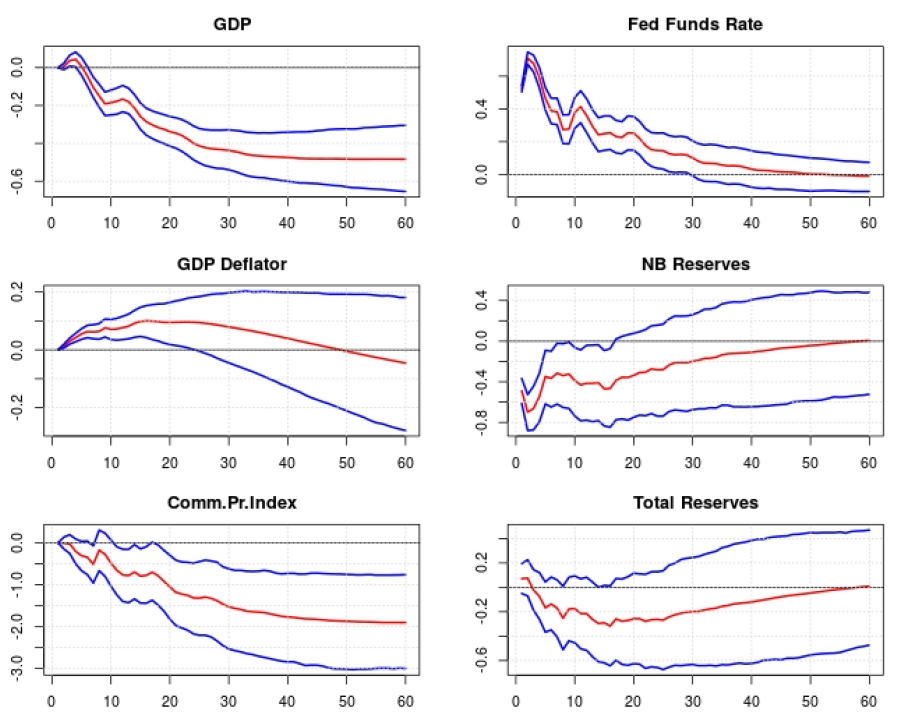
\includegraphics[width=0.7\linewidth]{irf uhlig.png}
    \end{figure}
\end{frame}





%======================================================
\begin{frame}{Example: Kilian (2009) "Not All Oil Price Shocks Are Alike"}
%======================================================
\scriptsize
Decompose movements in the real price of oil into economically meaningful structural shocks and study their macro effects.

\medskip
\textbf{3-variable monthly SVAR (global crude oil market):}
\[
z_t =
\begin{pmatrix}
\Delta \text{prod}_t \\ \text{rea}_t \\ \text{rpo}_t
\end{pmatrix}
\]
\begin{itemize}
  \item $\Delta \text{prod}_t$: growth rate of world crude oil production.
  \item $\text{rea}_t$: global real activity index in industrial commodity markets
        (constructed from dry bulk freight rates). 
  \item $\text{rpo}_t$: real price of crude oil.
\end{itemize}

\medskip
\textbf{Structural shocks:}
\begin{itemize}
  \item $\varepsilon^{\text{supply}}_t$: oil supply shock
        (unanticipated change in global oil production).
  \item $\varepsilon^{\text{agg.dem}}_t$: global aggregate demand shock
        (demand for all industrial commodities, driven by the world business cycle).
  \item $\varepsilon^{\text{prec}}_t$: oil-specific demand shock
        (\textbf{precautionary demand} for oil, reflecting uncertainty about future supply).
\end{itemize}

\medskip
\textbf{Identification (short-run recursive restrictions):}
\pause
\begin{itemize}
  \item Oil production does \textbf{not} respond contemporaneously to demand shocks.
  \item Real activity does \textbf{not} respond within the month to oil-specific shocks.
  \item Real oil price can respond immediately to all three shocks.
\end{itemize}
\end{frame}

\begin{frame}{Kilian (2009) IRFs'}
    \begin{figure}
        \centering
        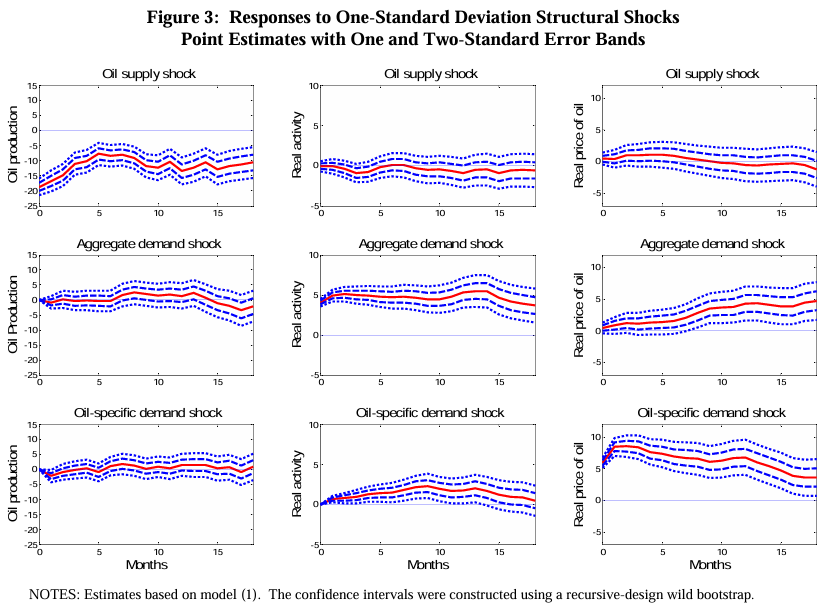
\includegraphics[width=1\linewidth]{irf killian.png}
    \end{figure}
\end{frame}
%======================================================
\begin{frame}{Kilian (2009) results 1/2}
%======================================================
\scriptsize
\textbf{IRFs for the oil market (key patterns):}
\begin{itemize}
  \item \textbf{Oil supply shock}: Small, short-lived fall in global oil production; only a \textbf{small and transitory} rise in the real price of oil; mild, temporary fall in global activity.
  \item \textbf{Aggregate demand shock}: Persistent increase in global real activity; \textbf{Large and sustained} increase in the real price of oil (with some delay).
  \item \textbf{Oil-specific (precautionary) demand shock}: \textbf{Immediate, sharp and persistent} rise in the real price of oil
                (with overshooting); Temporary drop in activity, little change in production. 
\end{itemize}

\medskip
\textbf{Historical decomposition of oil prices (1975-2007):}
\begin{itemize}
  \item For each shock $j$ the \textbf{contribution to the real price of oil} is:
  \[
    rpo_t^{(j)} = \sum_{h=0}^{H} \Psi_h(rpo,j)\, \varepsilon_{t-h}^{(j)}
  \]
  \item Setting $\varepsilon^{(j)}_t=0$ for all $t$:
        \textbf{counterfactual oil-price path without shock $j$}.
  \item Allow for \textbf{historical decomposition of oil-price movements}.
  \item $\Longrightarrow$ Oil price spikes arise mainly from \textbf{global aggregate demand}
        and \textbf{precautionary demand}, not supply shocks.
  \item The post-2003 surge is almost entirely driven by \textbf{world demand}.
\end{itemize}


\end{frame}



%======================================================
\begin{frame}{Kilian (2009): Historical Decomposition \& U.S. Macro Effects}
%======================================================
\footnotesize
\textbf{How the shocks are used?} The 3-variable oil-market SVAR provides \textbf{monthly structural shocks} $ \{\widehat{\varepsilon}^{supply}_t,\ \widehat{\varepsilon}^{agg.dem}_t,\ 
     \widehat{\varepsilon}^{prec}_t\}.$  \textbf{Not} U.S.-specific: they are global oil-market shocks!

\begin{itemize}
  \item Then estimates their macro effects using \textbf{external regressions / Local Projections} (next class):
  \[
  y_{t+h} = \alpha^h
  + \beta_1^h \widehat{\varepsilon}^{supply}_t
  + \beta_2^h \widehat{\varepsilon}^{agg.dem}_t
  + \beta_3^h \widehat{\varepsilon}^{prec}_t
  + \Gamma^h X_t + u_{t+h},
  \]
  where $y_{t+h}$ = U.S.\ GDP, CPI, IP, etc.
\end{itemize}


\textbf{Effects on U.S.\ macro variables (from the regressions):}
\begin{itemize}
  \item \textbf{Supply shocks}: small, temporary GDP drop; little CPI response.
  \item \textbf{Aggregate demand shocks}: initially raise GDP, later recessionary; CPI rises persistently.
  \item \textbf{Precautionary demand shocks}: stagflationary (GDP $\downarrow$, CPI $\uparrow$) (validate Bichler \& Nitzan, \textit{Capitalism as power}?)
\end{itemize}

"Oil price shocks" are not unique objects, their macro effects depend on
\textit{which} structural shock moved the oil price.
\end{frame}




%======================================================
\begin{frame}{Good practice for Cholesky identification}
%======================================================
\scriptsize

\textbf{1. Always justify the variable ordering!}
\begin{itemize}
  \item  Actually we impose a causal hierarchy: variables earlier in the list cannot react within the period \textbf{= substantive economic assumption}.
\end{itemize}

\pause

\textbf{2. Use the (longest) appropriate frequency.}
\begin{itemize}
  \item Cholesky assumes no contemporaneous reaction.
  \item More credible at quarterly frequency than monthly; rarely valid daily/weekly. Look at empirical/theoretical priors in the literature.
\end{itemize}

\pause
\textbf{3. Start with slow-moving variables.}
\begin{itemize}
  \item Put “sticky” variables first (real activity, employment).
  \item Put fast-moving policy variables last (interest rate, exchange rate, financial volatility).
\end{itemize}

\pause
\textbf{4. Check robustness to alternative orderings.}
\begin{itemize}
  \item Try several\textbf{ \emph{economically plausible} }orderings (e.g.\ $(g,\pi,i)$ vs.\ $(\pi,g,i)$) and report at least one alternative.
  \item If IRFs are broadly similar across these, your main results do not hinge on one arbitrary causal hierarchy (either contemporaneous correlations are modest ($\Sigma_u$ almost diagonal) or lag dynamics dominate the responses): reassuring.
  \item \textbf{If IRFs change a lot, conclusions are highly sensitive to the recursive assumptions} (i.e. data do not pin down a unique "shape" for contemporaneous responses): you must even more (i) justify the preferred ordering theoretically, and (ii) show how results vary under alternatives.
\end{itemize}

\end{frame}




%======================================================
\begin{frame}{Good practice for Cholesky identification}
%======================================================
\small

\textbf{5. Inspect the reduced-form residual covariance matrix.}
\begin{itemize}
  \item If variables are nearly collinear (all $\Sigma_u$ terms$\approx$ $1$), Cholesky numerically unstable. Possibly common shocks / a common latent factor.
  \item Check that $\hat\Sigma_u$ is well-conditioned. If ill-conditioned/non-invertible: not enough independent statistical variations. 
\end{itemize}

\medskip

\textbf{6. Cholesky = sufficient but \emph{not necessary}}

\medskip

\normalsize
\textbf{Other methods:}
\begin{itemize}
  \item more general short-run restrictions (recursive Cholesky decomposition is a special case) (Blanchard-Perotti),
  \item long-run restrictions (Blanchard-Quah),
  \item sign restrictions (Uhlig),
  \item narrative approach (Romer \& Romer, Ramey) 
  \item external instruments (Proxy-VAR).
\end{itemize}

\end{frame}















\section{Short-run rest}

%======================================================
\begin{frame}{Why shocks?}
%======================================================
\small
\begin{itemize}
  \item Large SVAR literature on \textbf{policy shocks}: monetary and fiscal.
  \item \textbf{Goal:} estimate the dynamic impact of \textbf{exogenous} fiscal/monetary shocks
        on $Y$ (output, unemployment, inflation, asset prices, \dots).
  \item Policy variables are typically \textbf{endogenous}:
        they react systematically to the state of the economy.
  \item Need to construct shocks that are \textbf{as exogenous as possible}:
        \begin{itemize}
          \item either from the VAR (identification),
          \item or from external information (laws, speeches, narrative, news).
        \end{itemize}
  \item Canonical example for \textbf{short-run restrictions}: \\
        Blanchard \& Perotti (2002, QJE) on \textbf{tax} and \textbf{government spending} shocks.
        \item Very hot topic during the period of fiscal consolidation in the euro area during the 2011-13 recession (sovereign-banking nexus), see Blanchard-Leigh (IMF WP, 2011) vs. Fazzari et al. (2014).
\end{itemize}
\end{frame}




\begin{frame}{Short-run (i.e. contemporaneous) restrictions}
\small
\textbf{Short-run restriction:} use institutional timing/information lags to rule out some \emph{within-period} responses.
\begin{itemize}
  \item Translate these timing assumptions into \emph{zero restrictions} on contemporaneous effects.
  \item Set selected elements in $B_0$ (or equivalently in $C(0)$) to zero to encode who can react contemporaneously to whom.
\end{itemize}

\textbf{Recursive (Cholesky): a special case!}
\begin{itemize}
  \item Earlier-ordered variables do not react contemporaneously to later-ordered ones, and later variables can react to earlier ones.
\end{itemize}

\textbf{Non-recursive short-run restrictions}
\begin{itemize}
  \item \textbf{Allow some pairs to interact contemporaneously while others do not} (e.g. \textit{\textbf{common shocks}})
  \item Encode richer institutional structures than a single ordering (e.g, financial variables jointly contemporaneous, but real variables slow).
  \item Appropriate when evidence suggests simultaneity among a subset of variables (no hierarchy).
\end{itemize}
\end{frame}

\begin{frame}{From timing assumptions to matrix zeros}
\small
\textbf{Economic timing assumptions}
\begin{itemize}
  \item Decision/implementation lags: some policies cannot change and/or affect macro variables within the same month/quarter.
  \item Information lags: agents do not observe certain contemporaneous variables when deciding.
  \item Adjustment frictions: prices/wages may not adjust within the period; financial variables do.
\end{itemize}

\textbf{Example:}
\begin{itemize}
  \item Example with two variables $(y_1, y_2)$ and shocks $(\varepsilon_1, \varepsilon_2)$:
  \[
    B_0 \begin{bmatrix} y_{1t} \\ y_{2t} \end{bmatrix} = \cdots + \begin{bmatrix} \varepsilon_{1t} \\ \varepsilon_{2t} \end{bmatrix}, 
    \quad
    B_0 = \begin{bmatrix} 1 & a_{12} \\ a_{21} & 1 \end{bmatrix}
  \]
  \item If $y_1$ cannot respond contemporaneously to $\varepsilon_2$, set $a_{12}=0$.
  \item The collection of such zeros defines the contemporaneous structure.
  \item   Overidentification: extra zeros are testable via likelihood ratio tests (but risk for no solution if data contradict)
\end{itemize}
\end{frame}

%======================================================
\begin{frame}{Example: Blanchard \& Perotti (2002)}
%======================================================
\small
BP estimate a quarterly reduced-form VAR:
\[
Y_t = A(L) Y_{t-1} + U_t
\]
where:
\begin{itemize}
  \item $Y_t = (T_t, G_t, X_t)'$:
  \begin{itemize}
    \item $T_t$: net taxes (real, per capita),
    \item $G_t$: government spending on goods and services,
    \item $X_t$: GDP.
  \end{itemize}
  \item $U_t = (t_t, g_t, x_t)'$: reduced-form residuals, with
        non-zero cross-correlations.
\end{itemize}

\medskip
\textbf{Identification problem:} express $U_t$ in terms of
\textbf{structural shocks}:
\[
(t_t, g_t, x_t)' = C(0)\,(e^T_t, e^G_t, e^X_t)',
\]
where:
\begin{itemize}
  \item $e^T_t$ = tax shock, $e^G_t$ = spending shock, $e^X_t$ = output shock, $C(0)$ the impact matrix (inverse of contemporaneous relation matrix $B_0$)
  \item and such that the $e$'s are mutually uncorrelated (structural).
\end{itemize}
\end{frame}

%======================================================
\begin{frame}{Short-run system for residuals}
%======================================================
\small
BP write an \textbf{explicit contemporaneous system}, \textit{\textbf{not }}for $B_0$ but directly for errors $C(0)e_t=U_t$:
\[
\begin{aligned}
t_t &= a_1 x_t + a_2 e^G_t + e^T_t \qquad (1) \\
g_t &= b_1 x_t + b_2 e^T_t + e^G_t \qquad (2) \\
x_t &= c_1 t_t + c_2 g_t + e^X_t \qquad (3)
\end{aligned}
\]

Interpretation?
\pause
\begin{itemize}
  \item Unexpected tax movement $t_t$ can come from:
  \begin{itemize}
    \item automatic response to GDP: $a_1 x_t$,
    \item contemporaneous reaction to a spending shock: $a_2 e^G_t$,
    \item \textbf{pure tax shock} $e^T_t$.
  \end{itemize}
  \item Unexpected spending $g_t$ can respond to GDP ($b_1 x_t$),
        to tax shocks ($b_2 e^T_t$), and to its \textbf{pure own shock} $e^G_t$.
  \item Unexpected output $x_t$ can react contemporaneously to taxes and spending
        (fiscal multipliers $c_1$ and $c_2$), plus its\textbf{ pure own shock} $e^X_t$.
\end{itemize}

\medskip
This is a system of \textbf{short-run (within-quarter) restrictions} on $C(0)$.
\end{frame}

%======================================================
\begin{frame}{Key quarterly assumptions (short-run restrictions)}
%======================================================
\small
BP separate two channels in $a_1$ and $b_1$:
\begin{enumerate}
  \item \textbf{Automatic stabilizers:} mechanical reaction under existing tax/transfer rules.
  \item \textbf{Discretionary policy}: active fiscal decision responding to the cycle.
\end{enumerate}

\medskip
\textbf{Main short-run assumptions (quarterly horizon), institutional information-grounded:}
\begin{itemize}
  \item Discretionary fiscal policy (channel 2) \textbf{cannot} respond
        within the quarter to unexpected GDP shocks (decision and implementation lags).
  \item So $a_1$ and $b_1$ capture \textbf{only automatic stabilizers} and can be set
        using \textbf{institutional elasticities}, not estimated from the VAR.
  \item Using OECD-based elasticities: $a_1 \approx 2.08$ (elasticity of taxes $i$ to their tax base $\times$ elasticity of tax base to GDP)
  \item  By looking at institutional information about govt purchases, they argue there is \textbf{no evidence} that they respond automatically to GDP within the quarter (channel 1) $\Rightarrow b_1 = 0$ (since both channels $=0$).
\end{itemize}
\end{frame}

%======================================================
\begin{frame}{Cyclically adjusted residuals and output equation}
%======================================================
\small
Given $a_1$ and $b_1$, they compute \textbf{cyclically adjusted} residuals:
\[
t'_t = t_t - a_1 x_t, \qquad
g'_t = g_t - b_1 x_t = g_t,
\]
so that $t'_t$ and $g'_t$ are (approximately) purged of automatic
responses to GDP.

\medskip
From (3):
\[
x_t = c_1 t_t + c_2 g_t + e^X_t.
\]

Because $t'_t$ and $g'_t$ no longer contain output shocks, they can be
used as \textbf{instruments} to identify $c_1$ and $c_2$:
\begin{itemize}
  \item regress $x_t$ on $t_t$ and $g_t$ using $(t'_t, g'_t)$ as instruments,
  \item obtain \textbf{contemporaneous output multipliers} of tax and spending shocks.
\end{itemize}

\medskip
Now we know how output reacts within the quarter to \textbf{pure} tax and spending shocks.
\end{frame}

%======================================================
\begin{frame}{Ordering between tax and spending shocks}
%======================================================
\small
The remaining parameters $a_2$ and $b_2$ describe cross-effects
between tax and spending shocks:
\[
t_t = a_1 x_t + a_2 e^G_t + e^T_t, \quad
g_t = b_1 x_t + b_2 e^T_t + e^G_t.
\]

\begin{itemize}
  \item There is no strong institutional reason to pin down $a_2$ vs.\ $b_2$.
  \item BP therefore consider two polar cases:
  \begin{enumerate}
    \item \textbf{Taxes decided first}: $a_2 = 0$, estimate $b_2$.
    \item \textbf{Spending decided first}: $b_2 = 0$, estimate $a_2$.
  \end{enumerate}
  \item In the data, the correlation between $t'_t$ and $g'_t$ is small, so both orderings give very similar results.
\end{itemize}

\medskip
$\Longrightarrow$ \textbf{non-recursive} short-run identification scheme: some elements of $C(0)$ are set using \textbf{institutional information} and elasticities.
\end{frame}

%======================================================
\begin{frame}{Empirical results}
%======================================================
\small
BP’s estimated contemporaneous multipliers (within quarter):

\begin{itemize}
  \item $c_2 > 0$: a one-unit spending shock increases GDP (around $1$ USD).
  \item $c_1 < 0$: a one-unit tax shock decreases GDP (around $0.8$-$0.9$ USD).
\end{itemize}

\medskip
\textbf{Dynamic IRFs:}
\begin{itemize}
  \item Tax shocks: negative, peak multipliers roughly between $-0.8$ and $-1.3$
        depending on the (DT vs.\ ST) specification.
  \item Spending shocks: positive, multipliers around $1$ / slightly above,
        with some persistence.
\end{itemize}

\medskip
\begin{itemize}
  \item \textbf{Signs consistent with standard theory}: higher spending $\Rightarrow$ higher GDP,
        higher taxes $\Rightarrow$ lower GDP.
  \item \textbf{Size and persistence depend on how trends/non-stationarity are treated} (Deterministic Trend DT (so detrending) vs. Stochastic Trend (i.e. trending random walk so first-difference)),
        but qualitative patterns are robust.
\end{itemize}
\end{frame}


\begin{frame}{IRF from a tax shock (DT vs. ST)}
    \begin{figure}
        \centering
        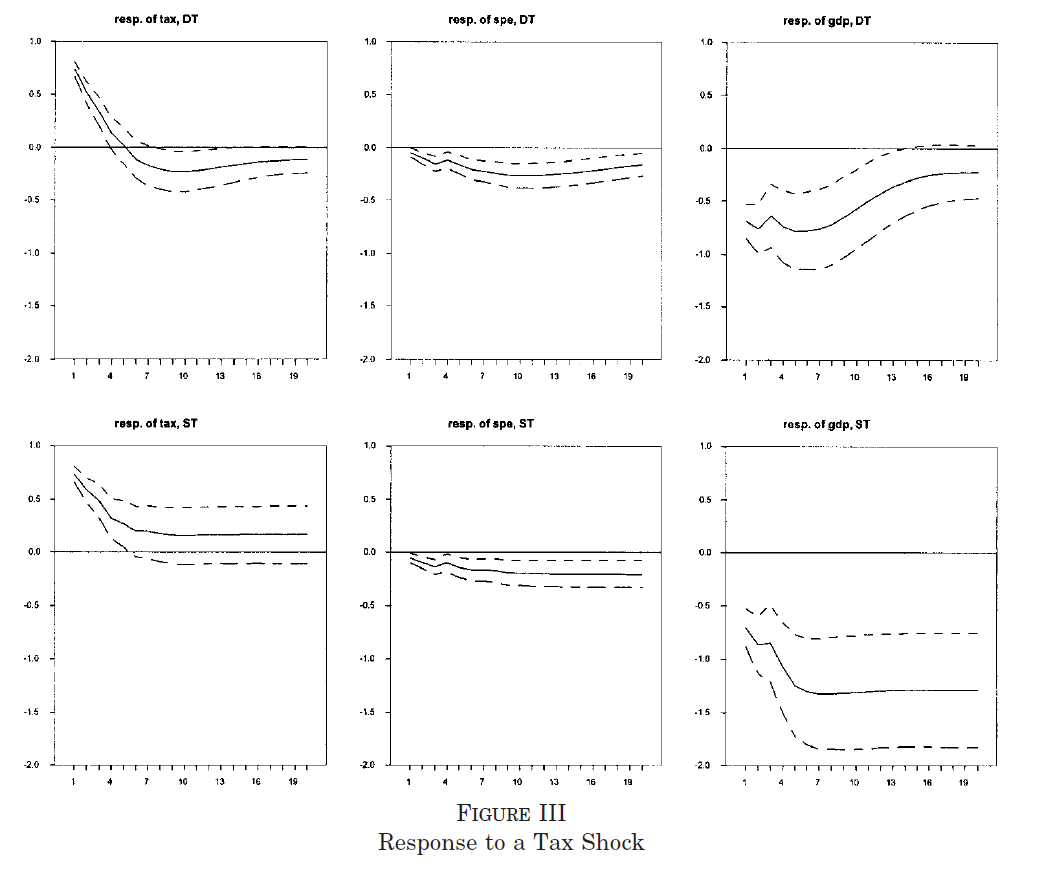
\includegraphics[width=0.9\linewidth]{IRF tax BP.png}
    \end{figure}
\end{frame}

\begin{frame}{IRF from a spending shock (DT vs. ST)}
    \begin{figure}
        \centering
        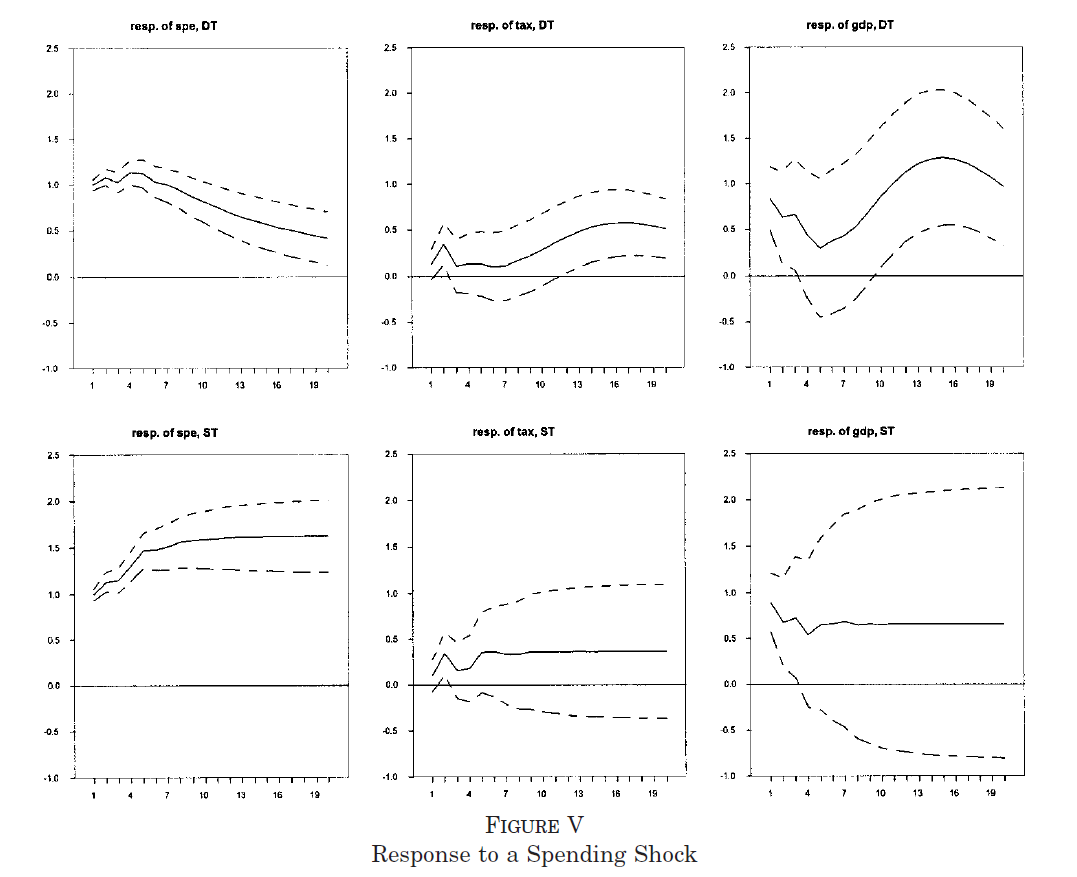
\includegraphics[width=0.9\linewidth]{IRF spending BP.png}
    \end{figure}
\end{frame}

















%======================================================
\section{Long-run rest}
%======================================================

%======================================================
\begin{frame}{Long-run restrictions}
%======================================================
\small
So far, short-run restrictions (e.g.\ Cholesky, Blanchard-Perotti):
\begin{itemize}
  \item Impose zeros (or other constraints) on \textbf{impact matrix} $C(0)$:
  \[
  u_t = C(0)\varepsilon_t, \quad \Sigma_u = C(0)C(0)'
  \]
  \item They control \textbf{contemporaneous} responses (within-period).
\end{itemize}

\medskip
\textbf{Long-run restrictions (seminal paper: Blanchard \& Quah, 1989)}:
\begin{itemize}
  \item Impose zeros (or other constraints) only on the \textbf{cumulative effect of shocks}:
  \[
  \text{long-run effect of shock } j \text{ on variable } i
  = \sum_{h=0}^{\infty} \Psi_h(i,j)
  \]
  \item Typical economic idea: some shocks are \textbf{transitory} (no effect on trend/level), others are \textbf{permanent}. 
  \item So need \textbf{at least one stationarized $I(1)$} series! Otherwise, no permanent shock!
\end{itemize}
\end{frame}



%======================================================
\begin{frame}{Long-run effects in the VAR representation}
%======================================================
\tiny
Reduced-form VAR($p$):
\[
y_t = \mu + A_1 y_{t-1} + \cdots + A_p y_{t-p} + u_t,
\quad \mathbb{E}[u_t u_t'] = \Sigma_u.
\]

Again, if the VAR is stable it has a VMA($\infty$) representation:
\[
y_t = \mu + \sum_{h=0}^{\infty} \Phi_h u_{t-h}, \qquad \Phi_0 = I_k
\]

\medskip
\textbf{Long-run effect of reduced-form shocks:}
\[
\Theta \equiv \sum_{h=0}^{\infty} \Phi_h
\]

Using lag polynomials, one can show:
\[
\Theta = \big(I_k - A_1 - \cdots - A_p\big)^{-1}
\quad\text{(if this inverse exists)}
\]

\medskip
With structural shocks $u_t = C(0)\varepsilon_t$, the structural MA is
\[
y_t = \mu + \sum_{h=0}^{\infty} \Psi_h \varepsilon_{t-h},
\qquad \Psi_h = \Phi_h C(0)
\]

\textbf{Long-run effects of structural shocks:}
\[
\Lambda \equiv \sum_{h=0}^{\infty} \Psi_h = \Theta\, C(0)
\]
Each column $j$ of $\Lambda$ gives the long-run effect of shock $j$ on all variables.
\end{frame}

%======================================================
\begin{frame}{Identification via long-run restrictions}
%======================================================
\scriptsize
We observe:
\[
A_1,\dots,A_p,\ \Sigma_u
\quad\Rightarrow\quad
\Theta = \big(I - A_1 - \cdots - A_p\big)^{-1}.
\]

We want $C(0)$ and $\varepsilon_t$ such that:
\[
\Sigma_u = C(0)C(0)', \qquad \Lambda = \Theta C(0)
\]
and some entries of $\Lambda$ are fixed by theory:
\[
\Lambda(i,j) = 0 \quad \text{(shock $j$ has no long-run effect on variable $i$)}
\]

\medskip
\textbf{Procedure (conceptually):}
\begin{enumerate}
  \item Estimate VAR $\Rightarrow$ $\hat A_i$, $\hat\Sigma_u$, $\hat\Theta$.
  \item Compute \textbf{long run var-cov matrix} $\hat\Omega = \hat\Theta\, \hat\Sigma_u\, \hat\Theta'$.
        Note: $\hat\Omega = \Lambda \Lambda'$.
  \item Choose \textbf{long-run impact matrix} $\Lambda$ to satisfy:
        \begin{itemize}
        %======================================================
\scriptsize
          \item $\Lambda \Lambda' = \hat\Omega$
          \item plus \textbf{long-run zero restrictions} (e.g.\ impose some entries of $\Lambda$ to zero).
        \end{itemize}
  \item Recover $C(0)$ from $\Lambda = \Theta C(0)$:
        \[
        C(0) = \Theta^{-1} \Lambda
        \]
\end{enumerate}

\medskip
$\Rightarrow$ as with short-run restrictions, we need $\frac{k(k-1)}{2}$ independent
long-run constraints to pin down $C(0)$. If $2\times2$, $\Sigma_u$ yields 3 restrictions, and a long-run one must be the 4th. No need for triangular $\Sigma_u$!
\end{frame}
\subsection{}
%======================================================
%======================================================
\begin{frame}{Example: Blanchard-Quah (1989)}
%======================================================
\footnotesize
The goal is to decompose \textbf{output fluctuations} into \textbf{supply} vs \textbf{demand}
shocks.

\medskip
2-variable VAR:
\[
y_t =
\begin{pmatrix}
\Delta y_t \\ u_t
\end{pmatrix}
\]
where $\Delta y_t$ is output growth and $u_t$ is unemployment.

\medskip
Structural interpretation:
\begin{itemize}
  \item Shock 1: \textbf{supply shock} (technology, productivity).
  \item Shock 2: \textbf{demand shock} (aggregate demand, monetary policy, etc.).
\end{itemize}

\medskip
\textbf{Key long-run restriction:}
\begin{itemize}
  \item Demand shocks have \textbf{no long-run effect} on the \textbf{level of output}.
  \item Since $\Delta y_t$ is \textbf{growth}, this means the \textbf{\emph{cumulative}} effect of a demand
        shock on $\Delta y_t$ is zero. In matrix notation, the long-run structural impact matrix
        \[
        \Lambda \;\equiv\; \sum_{h=0}^{\infty} \Psi_h \;=\; \Psi(1)
        =
        \begin{pmatrix}
        \lambda_{11} & \color{red}{0} \\
        \lambda_{21} & \lambda_{22}
        \end{pmatrix}
        \]
  \item Supply shocks can have a permanent effect on output.
\end{itemize}

This single long-run zero restriction, plus orthogonality, is enough to identify
demand vs.\ supply shocks in a 2-variable system.
\end{frame}

\begin{frame}{BQ's IRF from positive Supply shock}
    \begin{figure}
        \centering
        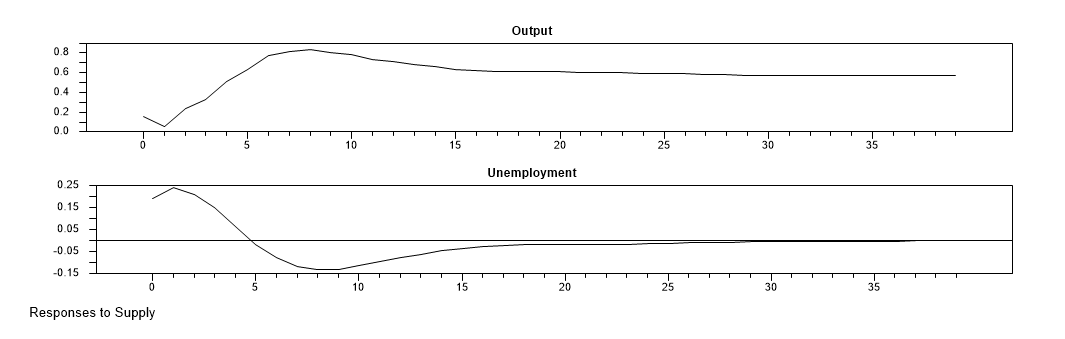
\includegraphics[width=1.1\linewidth]{BQ IRF 1.png}
    \end{figure}
\end{frame}




\begin{frame}{BQ's IRF from positive Demand shock}
\begin{figure}
    \centering
    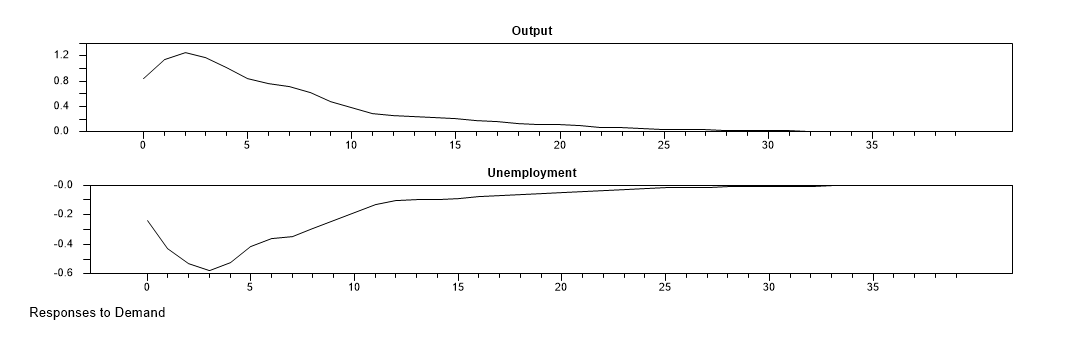
\includegraphics[width=1\linewidth]{irf bq demand.png}
\end{figure}
\end{frame}








%======================================================
\begin{frame}{Another example: technology shocks à la Galí (1999)}
%======================================================
\footnotesize
\textbf{Question:} What is the effect of \textbf{technology shocks} on hours worked?

\medskip
VAR with variables such as:
\[
y_t =
\begin{pmatrix}
\Delta (Y_t / N_t) \\ \Delta N_t \\ \dots
\end{pmatrix}
\]
where $Y_t/N_t$ is labour productivity, $N_t$ is hours (or employment).

\medskip
Structural interpretation:
\begin{itemize}
  \item Shock 1: \textbf{technology shock}.
  \item Shock 2: \textbf{non-technology shocks} (demand, policy, etc.).
\end{itemize}

\medskip
\textbf{Long-run restriction:}
\begin{itemize}
  \item Only technology shocks can affect the \textbf{long-run level of productivity}.
  \item Non-technology shocks have \textbf{zero long-run effect} on $Y_t/N_t$:
  \[
  \sum_{h=0}^{\infty} \Psi_h\big(\Delta (Y/N),\ \text{non-tech}\big) = 0
  \]
\end{itemize}
\end{frame}


%======================================================
\begin{frame}{Results}
%======================================================
\small
\textbf{Blanchard \& Quah (1989)}  
\begin{itemize}
  \item Demand shocks $\rightarrow$ hump‐shaped output rise, unemployment fall; effects fade in 3-5yrs.  
  \item Supply shocks $\rightarrow$ output effect builds over 2 yrs, plateaus 5 yrs; unemployment may rise initially.  
  \item Variance‐decomp: demand shocks contribute to 40-95\% of output volatility at 1-yr horizon (wide interval).  
\end{itemize}

\medskip

\textbf{Galí (1999)}  
\begin{itemize}
  \item Positive technology (permanent) shock $\rightarrow$ output $\uparrow$, hours $\downarrow$ (short‐/medium‐run).  
  \item Technology shock’s variance contribution to output/hours is\textbf{ modest; non‐tech (demand) shocks dominant.  }
  \item Evidence \textbf{challenges standard RBC} where hours $\uparrow$ after productivity shock.  
\end{itemize}
\end{frame}


%======================================================
\begin{frame}{Limits}
%======================================================
\small

\textbf{Limits:}
\begin{itemize}
  \item Require strong assumptions on the \textbf{trend properties} of variables
        (unit roots, cointegration, etc.). At least one stationarized but originally $I(1)$ series to allow for permanent shocks.
  \item Implicitly assume that the long-run restriction is \textbf{exactly true}
        (e.g.\ demand / money never change long-run output). \textbf{Ridiculously strong!}
        \item e.g. Fatas and Summers, JIE 2018, \textbf{\textit{The permanent effects of fiscal consolidations}}
        \item Why would cyclical components (Business / Financial cycles) \textit{not} have a long-run effect on trend? \textit{Structural change} (cf. Pasinetti, Schumpeter, Harvey, Goodwin's late work).

\end{itemize}

\medskip
But still another way to use \textbf{economic structure} (timing vs permanence) to select one structural model among many reduced forms.
\end{frame}



%======================================================
\begin{frame}{NB: the persistence of the effects of crises!}
%======================================================
\small
Measuring the effects of crises: effect on output (\textit{Growth Dynamics: The Myth of Economic Recovery)} Cerra \& Saxena, AER 2008 (estimate impulse response functions (IRFs) following a crisis, 190 countries, over the period 1960-2001): widening output (level) loss.

• Recessions induced by the financial cycle are longer and deeper, and can even have a permanent effect on the level of output, not just on growth (also BCBS, 2010; Claessens et al. 2012; Drehmann et al. 2017)
\begin{figure}
    \centering
    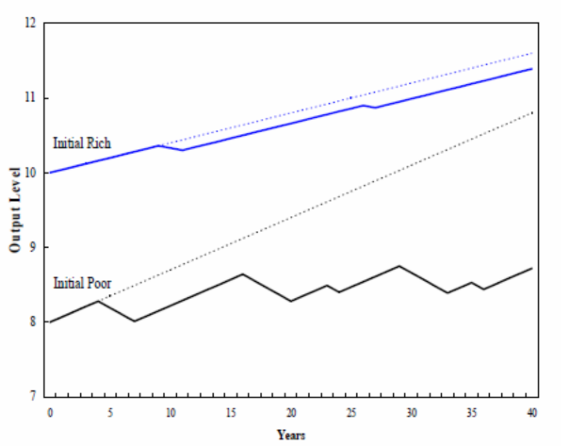
\includegraphics[width=0.55\linewidth]{crisis long effect.png}
\end{figure}
\end{frame}


















%======================================================
\section{Sign rest}
%======================================================

%======================================================
\begin{frame}{Sign restrictions?}
%======================================================
\small
\textbf{So far:}
\begin{itemize}
  \item \textbf{Short-run} (zero) restrictions: fix entries of $C(0)$ or $B_0$ (recursive / Cholesky, BP, etc.).
  \item \textbf{Long-run} restrictions: fix entries of $\Lambda = \sum_{h=0}^\infty \Psi_h$ (Blanchard-Quah).
\end{itemize}

Both require \textbf{exact zeros} and often strong functional assumptions.

\medskip
\textbf{Idea of sign restrictions (most well-known: Uhlig, 2005):}
\begin{itemize}
  \item Theory often delivers the \textbf{sign} of certain responses, not their exact size or timing.
  \item Impose that selected IRFs have the \textbf{right sign} over some horizons after a shock:
  \[
  \Psi_h(i,j) \ge 0 \quad\text{or}\quad \Psi_h(i,j) \le 0
  \]
  for chosen variables $i$, shocks $j$, horizons $h \in \mathcal{H}$.
  \item So no exact zeros (less parametric, more "agnostic")
\end{itemize}
\end{frame}



%======================================================
\begin{frame}{Structural VAR and sign restrictions}
%======================================================
\small
AGAIN (!) if the VAR is stable, there is a VMA($\infty$):
\[
y_t = \mu + \sum_{h=0}^{\infty} \Phi_h u_{t-h}
    = \mu + \sum_{h=0}^{\infty} \Psi_h \varepsilon_{t-h},
\quad
\Psi_h = \Phi_h C(0)
\]

\medskip
\textbf{Sign restrictions = inequality constraints on $\Psi_h$:}
\[
\Psi_h(i,j) \gtreqless 0
\quad\text{for selected } (i,j,h)
\]

Goal: \textbf{find} $C(0)$ (and hence structural $\varepsilon_t$) such that:
\[
\Sigma_u = C(0)C(0)',
\quad
\mathbb{E}[\varepsilon_t \varepsilon_t']=I_k,
\quad
\text{and the sign restrictions on } \Psi_h \text{ hold}
\]
\end{frame}

%======================================================
\begin{frame}{Rotations and set identification}
%======================================================
\small
You remember that without restrictions, $\Sigma_u$ as an infinite number of valid decomposition into a diagonal 
$\Sigma_\varepsilon$ (identity $I_k$ if normalized for unit variance). So from $\Sigma_u$, pick any factorisation, e.g. \textbf{Cholesky} (\textbf{but whatever since it will then rotate!})
\[
\Sigma_u = P P'
\]

Any orthogonal matrix $Q$ (i.e. matrix such that $Q'Q = QQ' = I_k$ so just rotation) yields:
\[
C(0) = P Q,
\quad
u_t = C(0)\varepsilon_t = P Q \varepsilon_t
\]

\medskip
Hence, for all imaginable matrix $Q$ (it's valid since just a rotation):
\[
\Psi_h = \Phi_h C(0) = \Phi_h P Q
\]

\textbf{Sign restrictions:} we select a \emph{subset} of orthogonal matrices:
\[
\mathcal{Q}^* = \big\{Q \in \mathbb{R}^{k\times k} \,:\,
Q'Q=I_k,\; \Psi_h(i,j)=\Phi_h P Q \text{ satisfies all sign constraints} \big\}
\]

\medskip
\begin{itemize}
  \item  Give a \textbf{set}\textbf{ of admissible $Q$ (\textit{"set identification"}), }not a single one!
  \item  Can summarise IRFs by e.g.\ median and credible bands across $\mathcal{Q}^*$.
\end{itemize}
\end{frame}



%======================================================
\begin{frame}{Sign restrictions, observational equivalence \& set identification}
%======================================================
\small
\textbf{Example in a $2\times2$ VAR (output $y_t$, prices $p_t$).}

\begin{columns}[T]
\column{0.48\textwidth}
\textbf{Bad scheme (too weak):}
\[
\text{Demand: } (+,+), \quad
\text{Supply: } (+,+)
\]
\begin{itemize}
  \item Both shocks raise $(y,p)$. Swapping the two columns of $C(0)$ leaves $\Sigma_u$ and the sign scheme unchanged.
  \item $\Rightarrow$ shocks are \textbf{observationally equivalent} under the restrictions (you cannot tell which shock is which)
\end{itemize}

\column{0.48\textwidth}
\textbf{Better scheme (distinct patterns):}
\[
\text{Demand: } (+,+), \quad
\text{Supply: } (+,-)
\]
\begin{itemize}
  \item Demand: $y\uparrow$, $p\uparrow$.
  \item Supply: $y\uparrow$, $p\downarrow$.
  \item Columns of $C(0)$ now have \textbf{different sign signatures}, so fewer $Q$ are admissible.
\end{itemize}
\end{columns}

\end{frame}

%======================================================
\begin{frame}{Algorithm}
%======================================================
\small
\textbf{Step 1)} Estimate the reduced-form VAR $\Rightarrow$ $\hat A_i$, residuals $\hat u_t$, covariance $\hat\Sigma_u$.

\medskip
\textbf{Step 2)} Compute any factorisation of $\hat\Sigma_u$:
\[
\hat\Sigma_u = \hat P \hat P'
\quad\text{(e.g.\ Cholesky)}
\]

\medskip
\textbf{Step 3)} For many draws:
\begin{enumerate}
  \item Draw a random orthogonal matrix $Q$ (e.g.\ from the Haar measure on $O(k)$).
  \item Set $C(0) = \hat P Q$ and compute structural IRFs:
        \[
        \Psi_h = \hat\Phi_h C(0)
        \]
  \item \textbf{Check sign restrictions} on $\Psi_h(i,j)$ for all $(i,j,h)$ in your restriction set. If satisfied, \textbf{keep} $(C(0),\Psi_h)$ and \textbf{discard} the others.
\end{enumerate}

\medskip
\textbf{Step 4)} Use the collection of accepted IRFs:
\begin{itemize}
  \item plot pointwise median, the 16-84\% bands etc.
  \item i.e. all curves correspond to identified shocks consistent with the sign restrictions.
\end{itemize}
\end{frame}

\subsection{}
%======================================================
\begin{frame}{Example: Uhlig (2005)}
%======================================================
\small
VAR with US data (postwar), including:
\[
y_t = \text{GDP},\ \text{prices},\ \text{commodity prices},\ \text{nonborrowed reserves},\ \text{Fed funds rate},\dots
\]
\textbf{Goal:} identify a \textbf{contractionary monetary policy shock}.

\medskip
\textbf{Restrictions:}
\begin{itemize}
  \item Following a contractionary shock:
    \begin{itemize}
      \item short-term interest rate $\uparrow$ (Fed funds rate non-negative),
      \item monetary aggregate / nonborrowed reserves $\downarrow$,
      \item price level or inflation \textbf{not increasing} (no \textit{price puzzle. Sure?}),
    \end{itemize}
    for several quarters after the shock (e.g.\ horizons $h = 0,\dots,H$).
  \item \textbf{No restriction} on the response of real GDP:
        data decide whether output falls, rises, or is unchanged.
\end{itemize}

\medskip
\textbf{Qualitative findings:}
\begin{itemize}
  \item Price level falls only gradually.
  \item GDP response is ambiguous $\Rightarrow$ consistent with near-neutrality of monetary policy in many samples!
\end{itemize}
\end{frame}


\begin{frame}{Estimated MP shock using Sign restrictions}
\begin{figure}
    \centering
    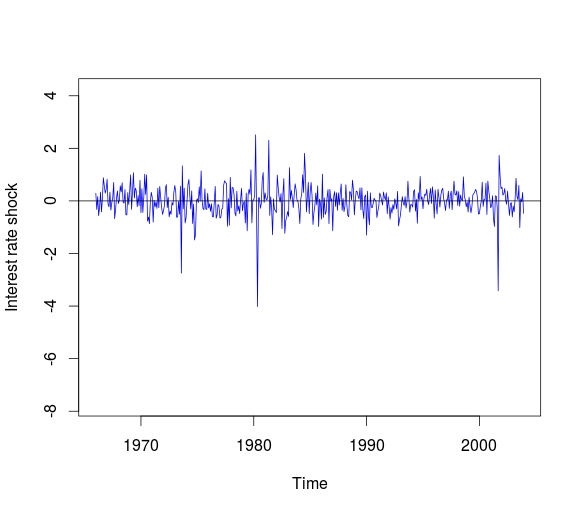
\includegraphics[width=0.8\linewidth]{Ulhig MP shocks.png}
\end{figure}
    
\end{frame}
\begin{frame}{Possible range of IRFs (Uhlig) with sign restrictions}
    \begin{figure}
        \centering
        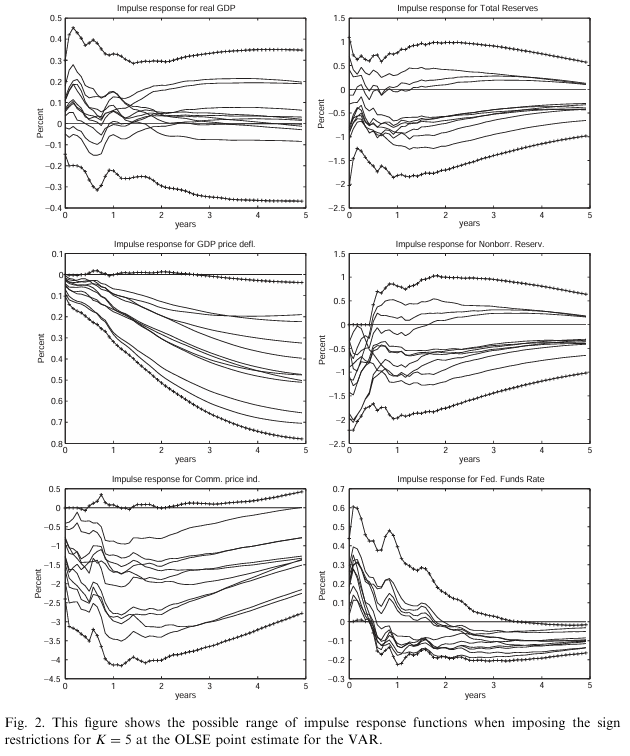
\includegraphics[width=0.65\linewidth]{Uhlig all IRF.png}
    \end{figure}
\end{frame}


\begin{frame}{Distribution of IRF with sign restrictions}
\begin{figure}
    \centering
    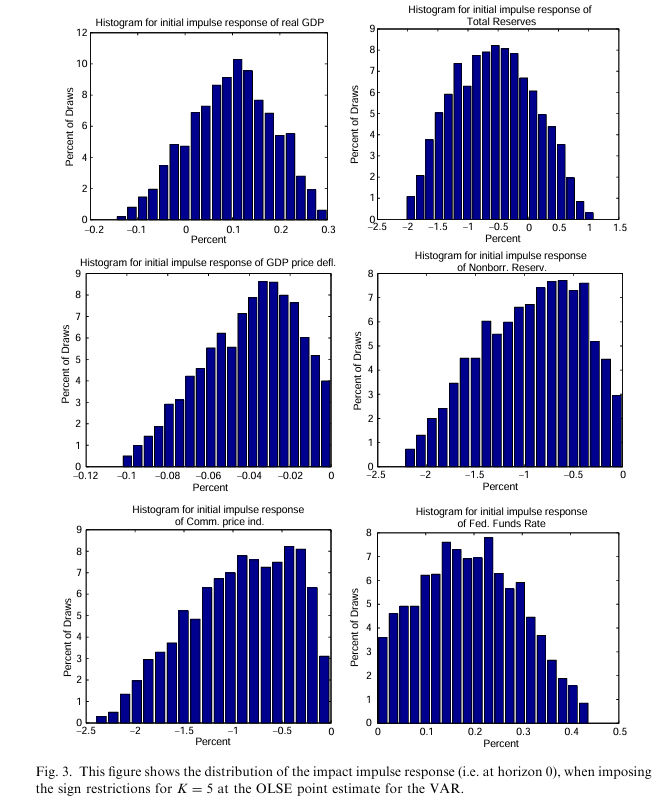
\includegraphics[width=0.65\linewidth]{Set of IRF with sign restriction.png}
\end{figure}
\end{frame}
\subsection{}
%======================================================
\begin{frame}{Pros and cons}
%======================================================
\small
\textbf{Advantages}
\begin{itemize}
  \item Weaker assumptions than zero short-run or long-run restrictions.
  \item Less sensitive to variable ordering (no recursive hierarchy encoded by construction).
  \item Direct way to make \textbf{theoretical \textit{qualitative} }predictions explicit in the IRFs.
\end{itemize}

\medskip
\textbf{Limitations}
\begin{itemize}
  \item Typically \textbf{set identification}: many admissible $C(0)$.
        $\Rightarrow$ IRFs are intervals, sometimes wide.
  \item Results can be sensitive to: 
        \begin{itemize}
          \item which variables are restricted,
          \item which horizons are constrained,
          \item whether "weak" sign restrictions (allow small violations) or not
        \end{itemize}
  \item Cannot easily impose "near-zero" responses (only sign, not magnitude).  But possible to do \textbf{bounds restrictions (e.g. for elasticities) }etc. 
  \item  Still a \textbf{theoretical} device: if the economic restrictions are mis-specified
        (e.g.\ they ignore the systematic policy rule), the identified ``shock'' may not be
        the structural shock you think it is (cf. Arias, Caldara \& Rubio-Ram\'{i}rez (2016) on Uhlig)!

\end{itemize}
\end{frame}


%======================================================
\begin{frame}{Why Uhlig (2005) finds almost no GDP effect? Methodological limits}
%======================================================
\scriptsize

\textbf{Uhlig's identification:} no restriction on GDP response (that's the point), BUT also NONE on the \textbf{systematic policy rule} (how $i_t$ reacts to $y_t,p_t,\dots$).
\begin{itemize}
\textbf{What Arias - Caldara - Rubio-Ramírez (2016) show:} contemporaneous policy equation:
  \[
  i_t = \psi_y y_t + \psi_p p_t + \psi_{pc} pc_t + \psi_{tr} tr_t + \psi_{nbr} nbr_t + \varepsilon^{mp}_t
  \]

  \item Under Uhlig's sign restrictions alone:
    \begin{itemize}
    \scriptsize
      \item posterior median $\psi_y \approx -0.43$, with $P(\psi_y<0)\approx 0.66$;
      \item $\psi_{tr},\psi_{nbr} \neq 0$ with probability $\approx 1$.
    \end{itemize}
  \item So most admissible models imply a \textbf{counterfactual rule}: Fed raises $i_t$ when $y_t$ falls and reacts to reserves.
\end{itemize}

\medskip
\textbf{Why this flattens / flips the GDP IRF (very concretely):}
\begin{itemize}
\scriptsize
  \item Because $\psi_y<0$, many ``MP shocks'' selected by the sign restrictions are actually
        \textbf{mixtures} of:
        \begin{itemize}
        \scriptsize
          \item a genuine rate hike \emph{plus}
          \item an underlying negative demand shock that already pushed $y_t$ down.
        \end{itemize}
  \item With such a rule, episodes where rates go up \textbf{while output is weak or falling are forced to be rationalised as “monetary shocks”}, because the rule would normally want to cut rates when $y$ increases.
    \item Those episodes typically occur in bad times (or with other shocks), so \textbf{GDP doesn’t fall much more}, or can even \textbf{rebound} overtime. 
\end{itemize}
\end{frame}


%======================================================
\begin{frame}{Fixing the issue: Arias - Caldara - Rubio-Ramírez (2016)}
%======================================================
\footnotesize
Averaging across all such admissible models $\Rightarrow$ median GDP IRF $\approx 0$ or $>0$
        $\Rightarrow$ \textbf{severe underestimation (even sign reversal) of the true contractionary effect.}

        \medskip
        
\textbf{Identification idea:}
\begin{itemize}
  \item Keep Uhlig's \emph{agnosticism on output}: no sign restriction on the IRF of $y_t$.
  \item Instead, discipline the \emph{systematic} policy rule:
    \begin{itemize}
    \footnotesize
      \item \textbf{Baseline:} fed funds reacts contemporaneously only to $y_t$ and $p_t$,
            with $\psi_y > 0,\; \psi_p > 0$, and $\psi_{tr} = \psi_{nbr} = 0$.
      \item \textbf{Alternative:} fed funds reacts only to money and commodity prices,
            $\psi_m > 0,\; \psi_y = \psi_p = 0$.
    \end{itemize}
\end{itemize}

\medskip
\textbf{IRFs:} in both schemes, a contractionary MP shock ($r_t\uparrow$) generates
\begin{itemize}
    \begin{itemize}
    \footnotesize
      \item a clear, hump-shaped fall in output,
      \item a decline (or at least no sustained rise) in the price level,
      \item a medium-run easing as policy systematically reacts to slowdown.
    \end{itemize}
\end{itemize}

\begin{itemize}
  \item Sign restrictions on IRFs alone can admit \emph{counterfactual} systematic policies,
        leading to misleading “monetary shocks”.
  \item Imposing\textbf{ restrictions on structural coefficients }(Baumeister \& Hamilton, 2015), \textbf{rather than IRF} might mitigate this drawback of set-identified SVARs. 
\end{itemize}

\end{frame}








\section{Narrative approach}


\begin{frame}{Narrative approach \& Identification}
\small

\begin{itemize}
\item In some circumstances, estimated shocks from SVARs may suffer from serious drawbacks
\item In particular, \textbf{omitted variable bias} is a central issue: policy actions and real economic activity are influenced by other variables not included in the SVAR.
\item \textbf{Idea: use a narrative approach that gathers systematic evidence from contemporaneous qualitative sources (newspapers, reports, policy transcripts).
} \pause
\item Other people usually call this \textit{"sociology"}.
\end{itemize}


\end{frame}

%======================================================
\begin{frame}{Why we need the \textbf{narrative approach}}
%======================================================
\footnotesize

Even if we try to recover the monetary policy shock by SVAR (e.g. Cholesky decomposition) with a standard backward-looking Taylor rule:
\[
\text{shock} \approx \text{(policy rate)} - \text{(systematic response)}
\]
i.e. the residuals of the estimated backward-looking Taylor rule (residuals $=$ \textit{non-systematic-rule part}) the approach remains \textbf{biased} for two reasons:

\medskip
\textbf{1. We rarely observe the central bank’s full information set}
\begin{itemize}
  \item CB reacts to internal forecasts, risk assessments,
        financial stability concerns, political constraints etc.
  \item These variables are \textbf{not} in typical VARs or Taylor-rule regressions.
  \item Hence the residual still includes this information $\phi_z z_t$.
\end{itemize}

\medskip
\textbf{2. The econometrician may misspecify the rule $f(\Omega_t)$}
\begin{itemize}
  \item The true reaction function is not necessarily linear or constant over time.
  \item Preferences, targets, and models used by policymakers evolve (Volcker vs. Bernanke!)
  \item A misspecified $f(\cdot)$ means the residual ≠ shock.
\end{itemize}

\bigskip

\textbf{So, narrative solution!} to identify \textbf{policy actions intentionally unrelated to the state of the economy}.

\end{frame}




\begin{frame}{Narrative approach \& Identification}
\small

\begin{itemize}
\item Romer \& Romer (seminal paper 1989, 2023) read FOMC \textit{Minutes} to find dates of exogenous monetary policy decisions (episodes where the CB deliberately tightened/loosened policy for reasons \emph{not driven} by current or expected output)
\item Produce a time series of binary indicators of monetary shocks ($m_t \in \{-1,0,1\}$)
\end{itemize}

\textbf{How to use narrative shocks?} 3 alternatives:
\begin{itemize}
  \begin{enumerate}
  \item \textbf{Include it as an exogenous regressor (VARX) or as the shock in a
        Structural VAR block where the narrative equation is purely exogenous.}
  \item Use \textbf{Local Projection }(\textit{cf. next class}) equation of interest with narrative shock as structural shock and compute IRFs (Jordà, 2015).
  \item If the measurement is noisy: \textbf{use it as an instrument (Proxy-VAR}, cf. \textit{next class})
  \end{enumerate}
\item Methods 1 and 2 yield quite similar results, but LP allow for nonlinearities.
\end{itemize}

\end{frame}



\begin{frame}{Narrative approach \& Identification}
\small

\begin{itemize}
\item Approach used e.g. in oil shocks (Hamilton 2003, \textit{exogenous historical events} (em­bargoes, supply disruptions)) and fiscal shocks (Romer \& Romer 2010; Ramey 2011)
\item Fiscal shocks are generally anticipated: agents react at announcement, before implementation
\item Narrative approach computes fiscal shocks from external sources (media, reports)
\end{itemize}

\vspace{0.3cm}

\begin{itemize}
\item Ramey \& Shapiro (1998) use narrative approach for spending shocks
\item Focus on cases where \textit{Business Week} suddenly forecast large defense spending not related to U.S.\ economy
\item These forecast jumps capture \textbf{news about future spending} (true shock on expectations), not delayed spending flows (contract timing)
\item 3 episodes: Korean war (Jul 1950), Vietnam war (Feb 1965), Soviet invasion of Afghanistan (Jan 1980)
\item Ramey (2011) adds 9/11 (Oct 2009) to get 4 dates.
\end{itemize}

\end{frame}

\begin{frame}{Defense spending since WWII}
\begin{figure}
    \centering
    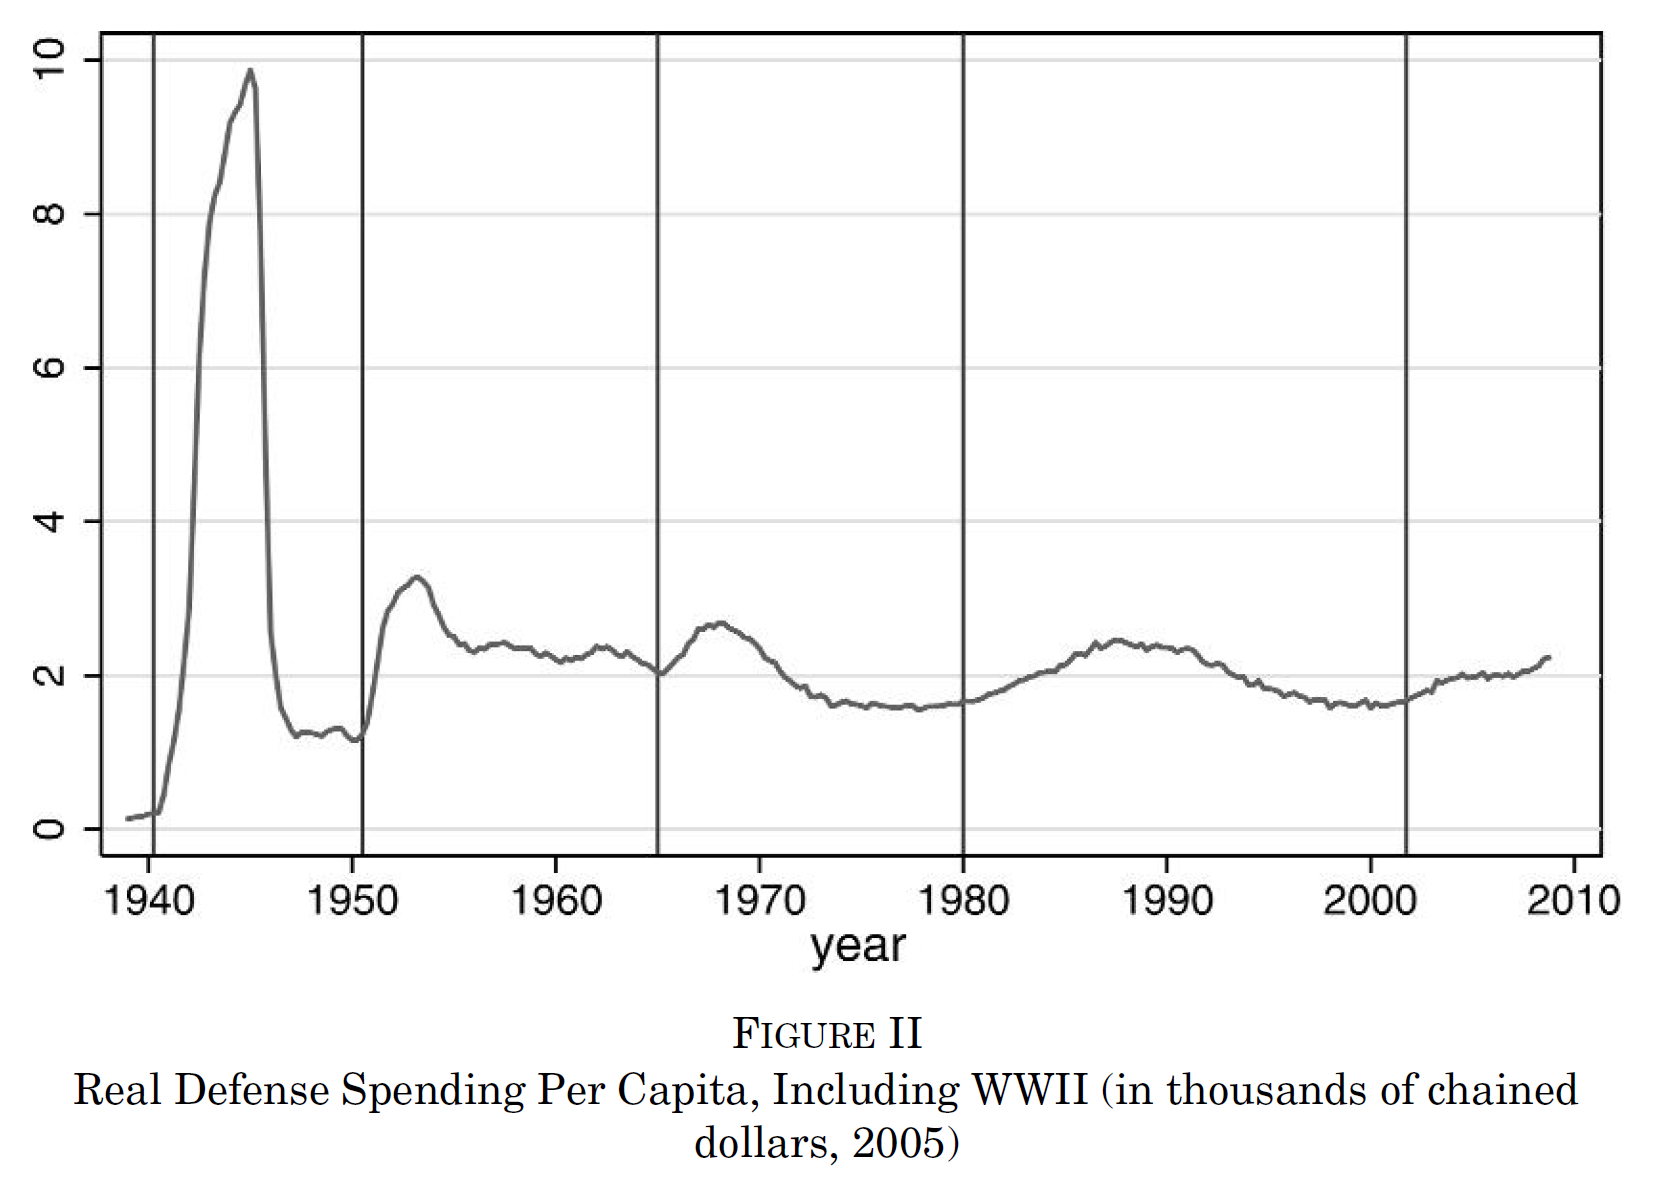
\includegraphics[width=1\linewidth]{def spending post ww2.png}
\end{figure}
    
\end{frame}


\begin{frame}{Narrative approaches: Ramey-Shapuro shocks}
    \begin{figure}
        \centering
        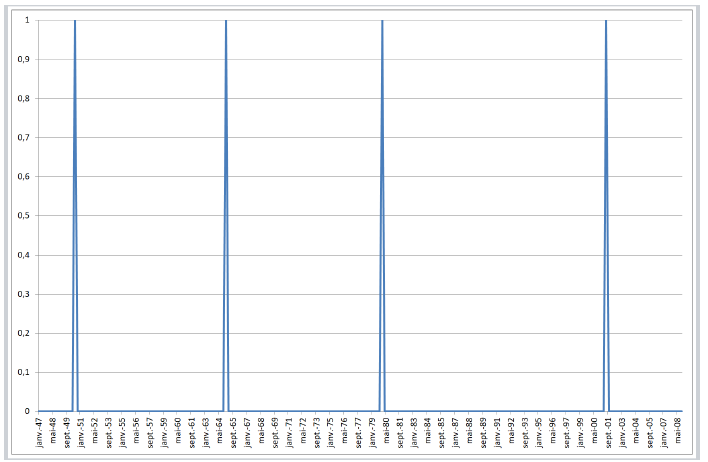
\includegraphics[width=1\linewidth]{ramey shapiro shocks.png}
    \end{figure}
\end{frame}




\begin{frame}{Narrative identification vs.\ Cholesky SVARs}
\scriptsize

Narrative identification uses \emph{historical information} (official records, newspapers, institutional documents) to date shocks that are plausibly exogenous.  


While Cholesky SVARs: identify shocks from \emph{statistical timing restrictions} (ordering -  $G$ ordered first $\Rightarrow$ its innovation is the spending shock.).

\vspace{0.3cm}

\textbf{1. Comparing impulse responses (general facts)}
\begin{itemize}
  \item If both approaches capture the same shock, IRFs should be similar.
  \item Differences reveal problems with (i) timing, (ii) anticipation, or (iii) the ordering assumption.
\end{itemize}

\textbf{Illustration: Ramey (2011)}
\begin{itemize}
  \item Govt spending, GDP, hours $\Longrightarrow$ similar (\textit{much stronger} rise for GDP \& H with narrative identification) $\Longrightarrow$ Because of expectations
  \item Consumption, investment, wages $\Longrightarrow$ opposite signs
\end{itemize}

\vspace{0.2cm}

\textbf{2. Granger-causality: diagnostic tool}
\begin{itemize}
  \item If \emph{narrative shocks} or \emph{professional forecasts} Granger-cause the SVAR shocks,  
        $\Rightarrow$ the SVAR shock is dated \emph{too late}.
  \item If SVAR shocks Granger-cause narrative shocks, $\Rightarrow$ narrative measure is incomplete or endogenous.
\end{itemize}

\textbf{Illustration: Ramey (2011)}
\begin{itemize}
  \item War-news shocks and SPF forecasts \emph{Granger-cause} the VAR "spending shocks", and the inverse if false. \textbf{Conclusion: VAR shocks are missing the timing of news} (delayed!)
\end{itemize}

\end{frame}


\begin{frame}{Narrative approaches: comparison of IRFs}
\begin{figure}
    \centering
    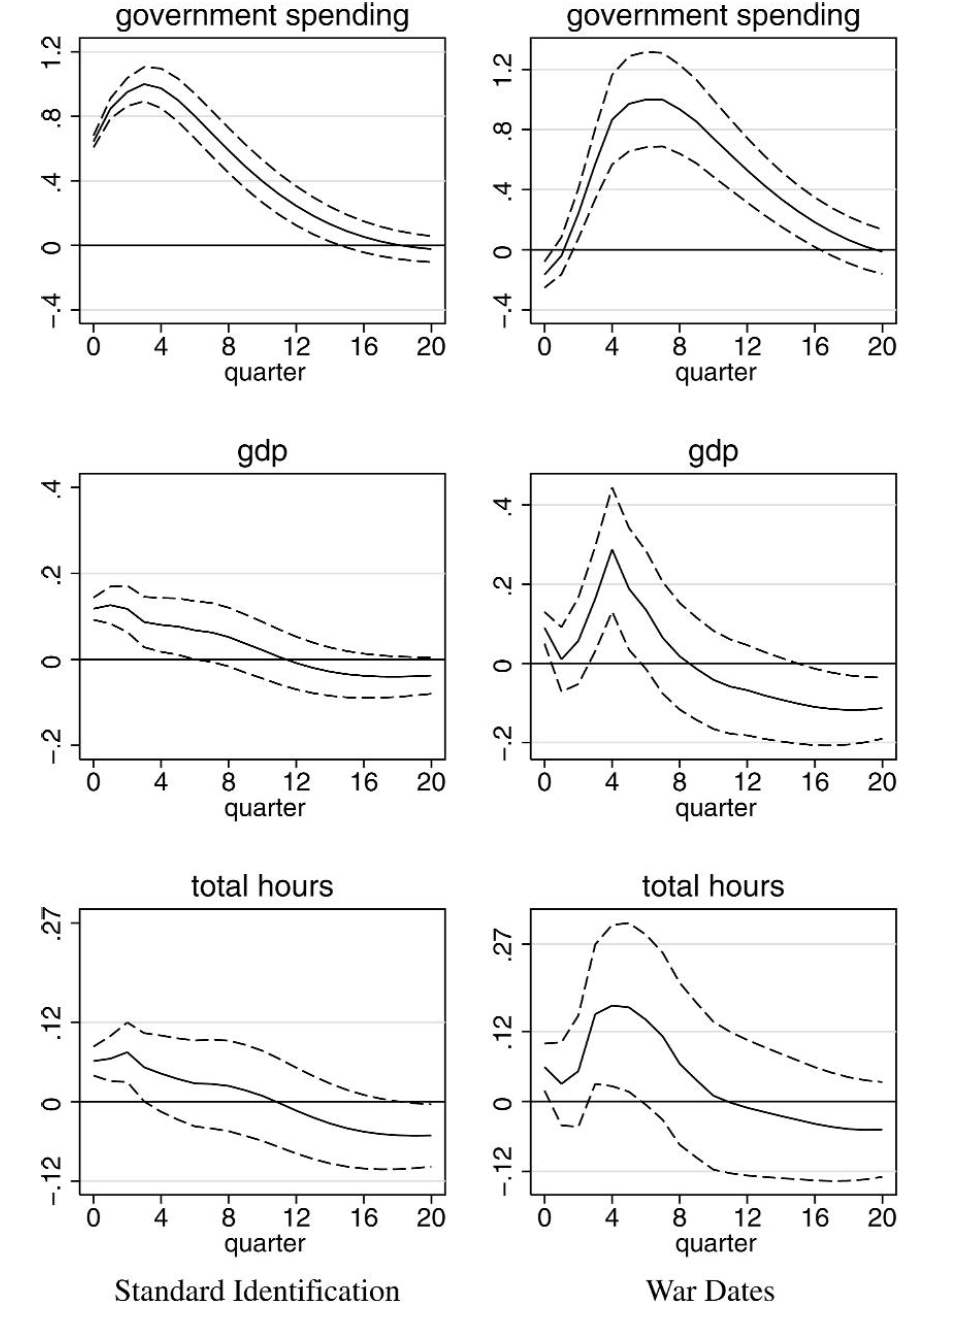
\includegraphics[width=0.5\linewidth]{RS IRF compa 2.png}
\end{figure}

    
\end{frame}



\begin{frame}{Narrative approaches: comparison of IRFs}
\begin{figure}
    \centering
    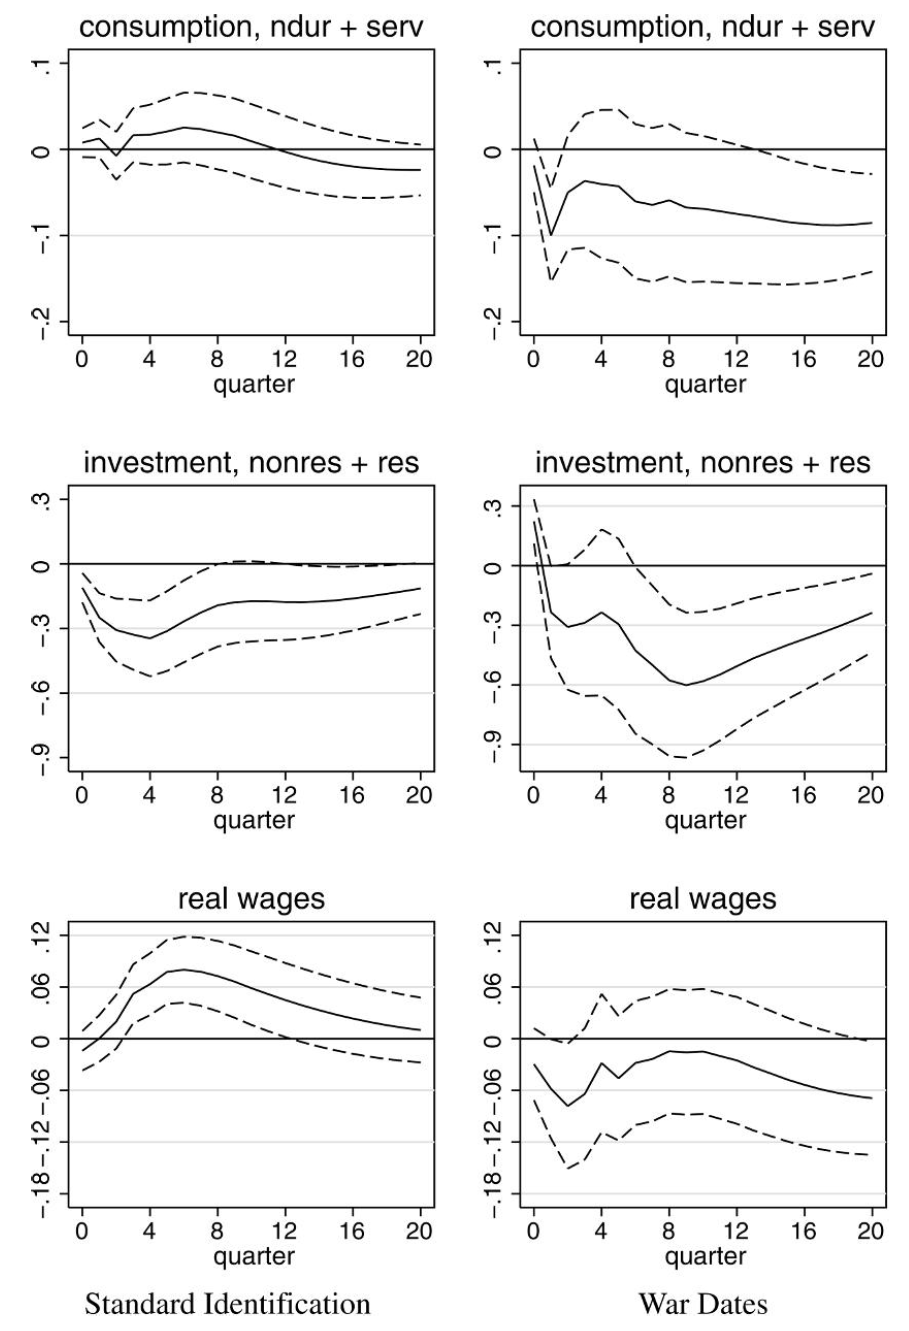
\includegraphics[width=0.5\linewidth]{RS IRF compa 1.png}
\end{figure}

    
\end{frame}


\begin{frame}{Granger causality (narrative approach)}
\begin{figure}
    \centering
    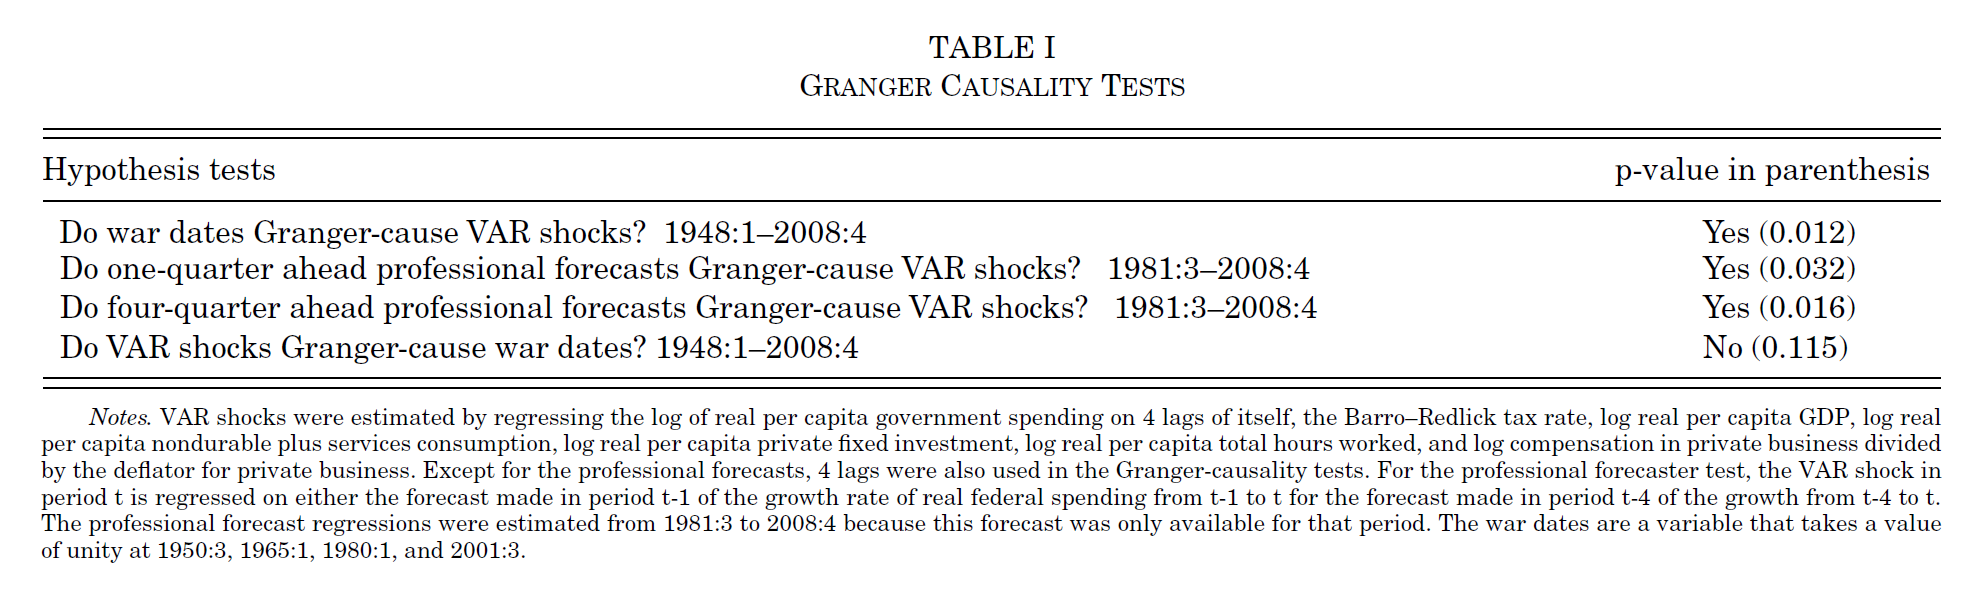
\includegraphics[width=1\linewidth]{RS Granger.png}

\end{figure}
\end{frame}



\section{Mon shocks}

\begin{frame}{Monetary policy shocks}
\small

\begin{itemize}
\item Monetary policy shocks are not easy to identify as there is strong endogeneity between macro activity and monetary policy: \textbf{Macro determines MonPol, which in turn affects Macro.}
\item Exogenous MP shocks are generally estimated using other data than the ones used in the SVAR, then they are integrated into the SVAR to assess dynamic macro effects.
\item Popular approach: Narrative identification of MP shocks, seminal paper by Romer and Romer (1989), revised version in 2023.
\item MP shock = MP is not driven by output or other factors affecting output, today and in the future.
\end{itemize}

\end{frame}



\begin{frame}{Monetary policy shocks}
\small

\begin{itemize}
\item More precisely, RR (1989) look for times when policymakers felt the economy was roughly at potential output but decided inflation was too high.
\item Policymakers then chose to cut money growth / raise interest rates, realizing there could be substantial negative consequences for aggregate output and unemployment.
\item In AS/AD terms: they look for times when the Fed deliberately shifted the aggregate demand curve back.
\end{itemize}

\vspace{0.4cm}

\begin{itemize}
\item In the new version, RR (2023) also estimate \textbf{expansionary} MP shocks.
\item They look for times when policymakers believed that they were at a stable level of economic activity, but took actions to lower unemployment and were willing to accept adverse consequences for inflation.
\item See examples of wording in the 2023 paper.
\end{itemize}

\end{frame}



\begin{frame}{Monetary policy shocks}
\centering

\textbf{Basically, a room for the sociology of institutions and public officials!}
\end{frame}


\begin{frame}{Requirements for a Narr App (RR, 2023)}
    \begin{figure}
        \centering
        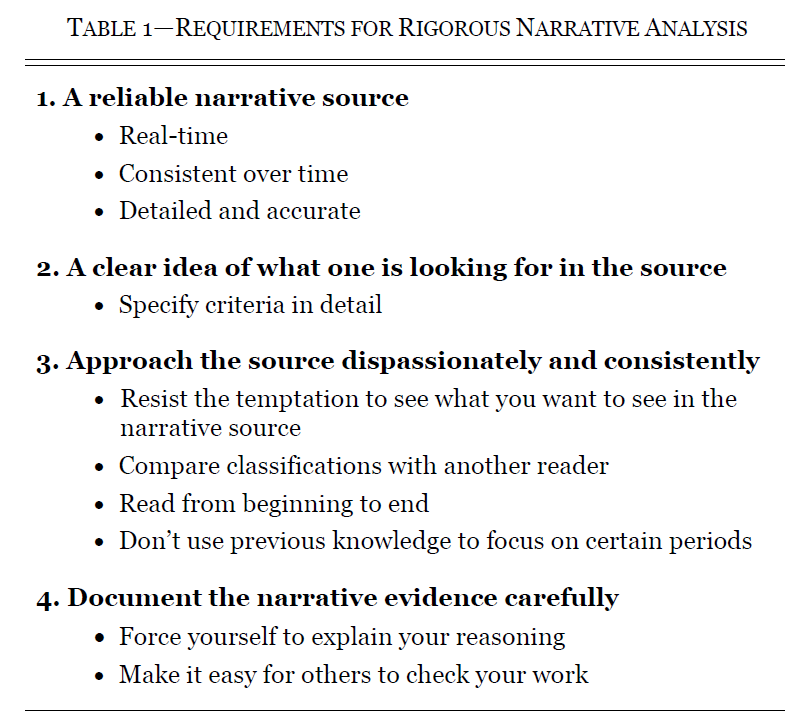
\includegraphics[width=0.8\linewidth]{RR requirements.png}

    \end{figure}
\end{frame}

\begin{frame}{RR (2023): dates of MP shocks}
    \begin{figure}
        \centering
        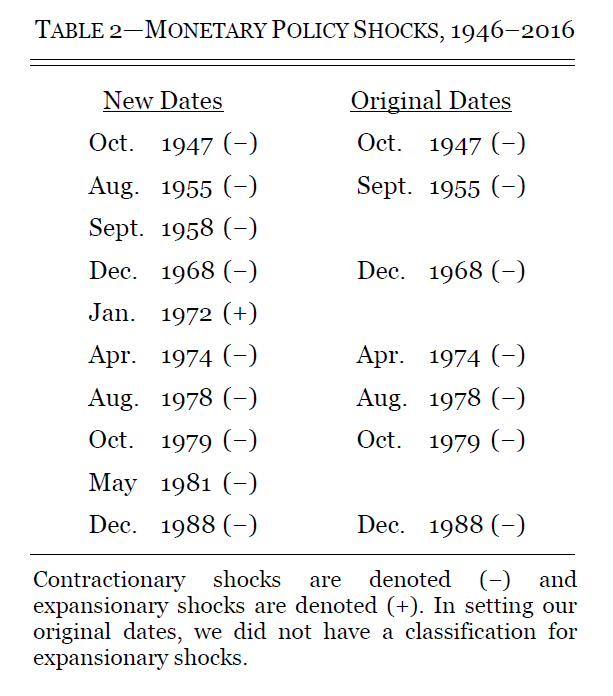
\includegraphics[width=0.6\linewidth]{RR dates MP shocks.png}
    \end{figure}
\end{frame}



\begin{frame}{Monetary policy shocks}
\small

\begin{itemize}

\item \textbf{Computation of the shock $m_t$} such that:
\[
m_t = 1 \text{ when contractionary MP shock at date } t,
\quad 
m_t = -1 \text{ when accommodative MP shock,}
\quad 
m_t = 0 \text{ otherwise.}
\]

\item \textbf{LP à la Jordà (2015) to assess IRF:}
\[
y_{t+h}
= \alpha^h + \beta^h m_t
+ \sum_{k=1}^K \theta_k m_{t-k}
+ \sum_{k=1}^K \phi_k y_{t-k}
+ u^h_{t+h}
\]

\item Sequence of estimated $\beta^h$ for horizons $h$ = IRF to a realization of $1$ of the MP dummy shock.

\vspace{0.35cm}

\item \textbf{Specification of the model:} $K = 12$ for monthly data; $K = 4$ for quarterly data.

\item \textbf{Sample size:} 1946-2016.

\item \textbf{Outcome variables:} Unemployment rate, GDP (level), Inflation (GDP deflator, PCE, Core PCE).

\end{itemize}

\end{frame}


\begin{frame}{RR (2023): IRF of UnempR to a MP shocks}
    \begin{figure}
        \centering
        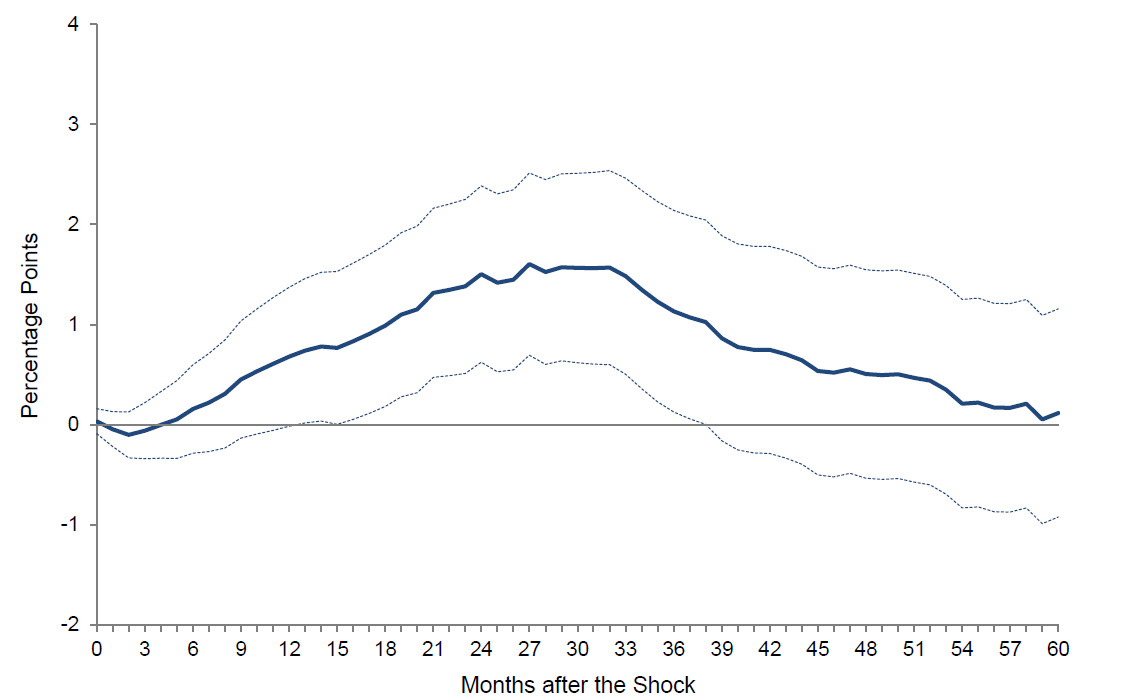
\includegraphics[width=1\linewidth]{RR 2023 IRF UNEMP.png}
    \end{figure}
\end{frame}

\begin{frame}{Comparison of shocks (IRF of GDP leaving out one shock}
\begin{figure}
    \centering
    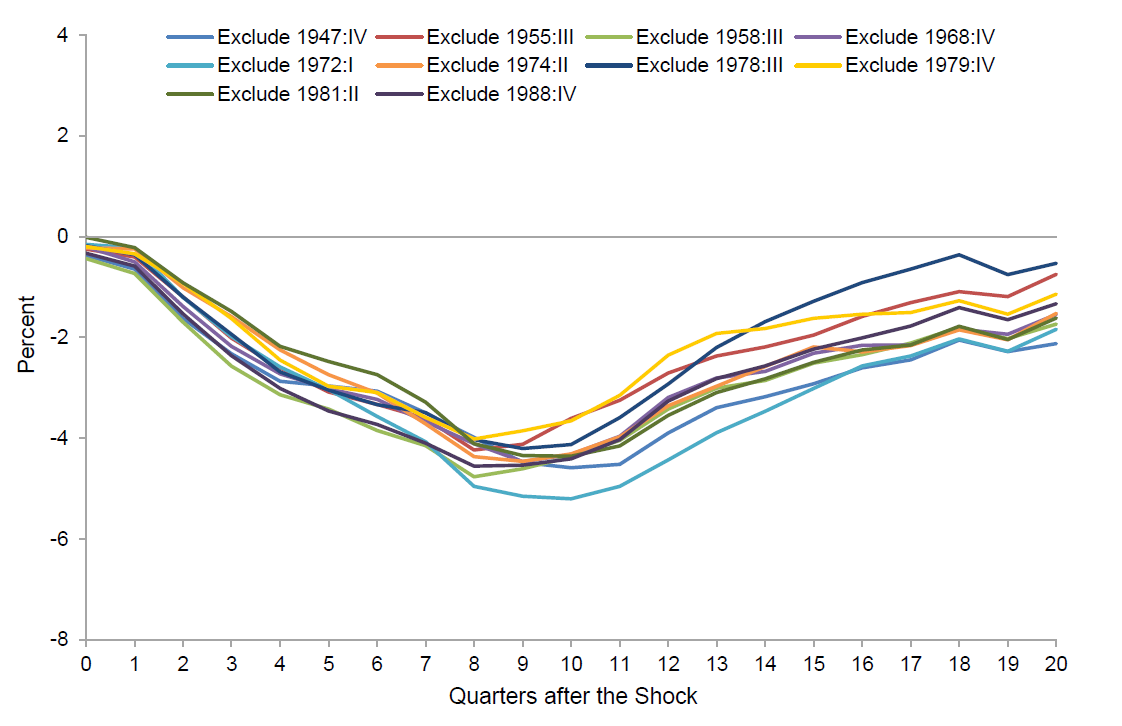
\includegraphics[width=1\linewidth]{IRF RR GDP one shock.png}
\end{figure}
    
\end{frame}




\begin{frame}{Monetary policy shocks: psychology and sociology of institutions}
\footnotesize

\begin{itemize}

\item Another way to compute MP shocks: changes in MP that are \textbf{orthogonal to the information that policy makers react to} (Romer \& Romer, 2004).

\item Policy instrument $s_t$ such that:
\[
s_t = f(\Omega_t) + \varepsilon_t
\]
$\Omega_t$: information set of the central bank, 
$f(\cdot)$: systematic component of MP, and $\varepsilon_t$ the MP shock.

\item $\varepsilon_t$ should be free of interest rate movements that are 
either endogenous responses to economic developments \textit{\textbf{or}} attempts 
by policy makers to counteract likely future developments (through info $\Omega_t$). They estimate:
\[
\Delta i_t = \alpha + \beta i_t + \gamma X_t^{f} + \varepsilon_t^{RR}
\]
where $i_t$ is the FFR and $X_t^{f}$ are forecasts of the CB made at time $t$.

\item Two key assumptions:
  \begin{enumerate}
  \footnotesize
  \item Forecasts must be a good proxy for the information set relevant
        for CB decisions (FOMC forecasts for the Fed).
  \item Mapping $f(\cdot)$ from the information to decisions is well
        approximated by a linear relationship.
  \end{enumerate}

\end{itemize}

\end{frame}





\begin{frame}{Monetary policy shocks}


\begin{itemize}

\item Extension of the RR (2024) approach by using more recent \textbf{machine learning techniques.}

\item Aruoba and Drechsel (2023) propose NLP \textbf{(Natural Language Processing}) to extract 
information from text (FOMC Minutes, number of certain specific words related to monetary policy).

\item Add textual information to the previous RR (2004) equation 
and allow for non-linearity in $f(\cdot)$.

\end{itemize}

\end{frame}


\section{Nonlin}

\begin{frame}{WHAT THE HECK ARE SHOCKS?}
\footnotesize

\pause

\footnotesize

More on this during classes on structural modelling, but a \textbf{critical issue} in \textit{mainstream} modelling!

\medskip

DSGEs need to assume (a LOT of) shocks to be identified (otherwise, \textit{stochastic singularity}).

\medskip

Real \textit{ontological} shocks (exogenous causes)? Or just th\textbf{e \textit{measure of our ignorance}?} (same question for the so-called "Solow's residual" - actually change in labour hoarding, in capacity utilization, in capital vintages etc)

\medskip

Shocks, or\textit{\textbf{ endogenous fluctuations from nonlinear dynamics}} thus not recognized by those linear specifications? 

\begin{figure}
    \centering
    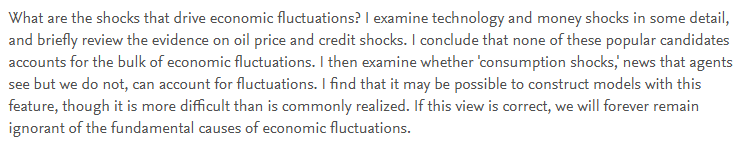
\includegraphics[width=1.1\linewidth]{Cochrane abstract.png}
    \caption{\footnotesize Abstract of "Shocks", John Cochrane (1994), NBER WP.}
\end{figure}

\end{frame}




%======================================================
\begin{frame}{Where we stand: linear VARs}
%======================================================
\footnotesize

So far, we have been working with \textbf{linear} macroeconometric systems:
\[
y_t = A_1 y_{t-1} + \cdots + A_p y_{t-p} + u_t,
\qquad u_t = C(0)\varepsilon_t
\]

\medskip
\textbf{Goals achieved:}
\begin{itemize}
  \item Forecasting and describing dynamic interactions (reduced-form VAR).
  \item Recovering \textbf{causal effects} of shocks (SVAR).
  \item Using identification strategies:
  \begin{itemize}
    \item recursive (Cholesky) short-run restrictions,
    \item long-run restrictions,
    \item sign / inequality restrictions,
    \item narrative shocks, proxy VARs (external instruments).%
    \footnote{\scriptsize In the \textbf{\Appendix} you will find two further strategies: \textbf{identification via heteroskedasticity} (Rigobon, 2003), and \textbf{max share identification} (Barksy \& Sims, 2011), than can be done also in the \textbf{spectral domain} (i.e.\ at given frequency bands) (Angeletos, Collard \& Dellas, 2020).}
  \end{itemize}
\end{itemize}

\medskip
\textbf{But all of this relies on a crucial assumption:}\\
\[
\text{{the data-generating process is \emph{linear}}}.
\]

\end{frame}


\begin{frame}{Impulse Response Functions (IRF) - Linearity}
\textbf{LIMITS OF LINEARITY}
\scriptsize
\smallskip
\begin{itemize}
    \item \textbf{As VARs are linear, a positive shock is the mirror image of a negative shock. }Only non-linear models can account for asymmetry.
    \begin{itemize}
    \scriptsize
        \item Always true in reality? \pause
        \item  Have the macro multipliers the same magnitude during expansion and during recession? E.g. Greek crisis (LMAO).
    \end{itemize}
    \item \textbf{As VARs are linear, the magnitude of the initial shock doesn’t matter in constructing the IRF.}
    \begin{itemize}
    \scriptsize
        \item Usually, a "unit shock" is a \textbf{one-standard-deviation shock} to the residual of a variable.
        \item 2.3 unit shock $\Longrightarrow$ 2.3 impulse response. 
        \item Always true in reality? \pause
        \item Thresholds? Tipping points? (e.g. the \textit{Great Moderation}, key rates and Minskyan moment). 
    \end{itemize}
     \pause
    \item \textbf{Stable linear VARs always converge to a unique equilibrium.}
    \begin{itemize}
    \scriptsize
        \item A stable VAR$(p)$ has MA($\infty$) form $y_t = \sum_{h=0}^{\infty} \Phi_h u_{t-h},\qquad \Phi_h \to 0 \text{ if stable}$
    \begin{itemize}
    \scriptsize
\item Hence if $\Phi_h \to 0$ (all eigenvalues $<1$):
    \end{itemize}
\[
\mathbb{E}[y_{t+h}\mid y_t] \to 0 \quad
(\text{or }\mu \text{ if not demeaned}).
 \]
        \item \textbf{Unstable linear VAR} ($|\lambda|\ge1$): $\Phi_h$ does not shrink → forecasts \textbf{explode}.
    \end{itemize}
\end{itemize}

\end{frame}



%======================================================
\begin{frame}{Nonlinear specifications?}
%======================================================

\textbf{Next class:}  

\medskip

When dynamics depend on the state of the economy, when IRFs change with the cycle, etc., we need \textbf{nonlinear} VARs.

\begin{itemize}
  \item threshold VARs,
  \item smooth-transition VARs,
  \item   Markov regime-switching VARs,
  \item Local Projections (with nonlinear terms),
  \item state-dependent IRFs.
\end{itemize}

\end{frame}







\appendix
\section{Appendix}



\begin{frame}{}

\Large

\centering 
\textbf{Appendix}

\end{frame}



\begin{frame}{Appendix: two further identification strategies}
\small

\textbf{We add two families of identification strategies.}


\begin{enumerate}\itemsep5pt
  \item \textbf{Identification through heteroskedasticity:} use changes in volatility regimes as extra moment conditions.
  \item \textbf{(Spectral) max share identification:} define the shock by what it explains most, either at a finite horizon or inside a frequency band (spectral approach).
\end{enumerate}

\medskip

\textbf{Same warning as always:} this is not assumption free (here, volatility stability or a variance dominance criterion).

\end{frame}


\begin{frame}{Identification through heteroskedasticity: intuition}
\small

Suppose the economy moves from a \textbf{quiet regime} to a \textbf{turbulent regime}.

\medskip

The reduced form residual covariance matrix changes:
\[
\Sigma_1 = \mathbb E(u_tu_t'\mid s_t=1),
\qquad
\Sigma_2 = \mathbb E(u_tu_t'\mid s_t=2).
\]

\medskip

If the \textbf{transmission matrix} from structural shocks to reduced form innovations is stable, but the \textbf{variances of structural shocks} change, then the second covariance matrix contains new information.

\medskip

\textbf{Key idea:} volatility changes rotate the covariance ellipse. If the shocks become more or less volatile by different relative amounts, this helps recover the structural directions.

\medskip

\footnotesize Rigobon (2003); Rigobon and Sack (2003, 2004); Sims and Zha (2006); Lütkepohl and Netšunajev (2021).

\end{frame}


\begin{frame}{Heteroskedastic SVAR: the basic algebra}
\small

Start from the reduced form VAR:
\[
y_t = A_1y_{t-1}+\cdots+A_py_{t-p}+u_t,
\qquad
u_t = B\varepsilon_t.
\]

\medskip

Let structural shocks be orthogonal within each regime:
\[
\mathbb E(\varepsilon_t\varepsilon_t'\mid s_t=r)=\Lambda_r,
\qquad
\Lambda_r \text{ diagonal}.
\]

\medskip

Then:
\[
\Sigma_r = \mathbb E(u_tu_t'\mid s_t=r)=B\Lambda_r B'.
\]

\medskip

Normalize regime 1 by scale, $\Lambda_1=I$. Then:
\[
\Sigma_1=BB',
\qquad
\Sigma_2=B\Lambda_2B'.
\]

\medskip

\textbf{So the same unknown matrix} $B$ \textbf{must explain \textit{two} covariance matrices, not only one.}

\end{frame}


\begin{frame}{Why this can identify the shocks}
\small

With the normalization $\Lambda_1=I$:
\[
\Sigma_2\Sigma_1^{-1}=B\Lambda_2B^{-1}.
\]

\medskip

Hence the columns of $B$ are the eigenvectors of $\Sigma_2\Sigma_1^{-1}$, and the eigenvalues are the relative volatility changes of the structural shocks.

\medskip

\textbf{Identification condition:}
\[
\lambda_i \neq \lambda_j \quad \text{for } i\neq j.
\]

\medskip

i.e.\ shock $i$ and shock $j$ must not have the same volatility ratio between the two regimes.

\medskip

\textbf{Economic meaning:} if every shock becomes twice as volatile in crisis, heteroskedasticity does not help. If financial shocks explode while technology shocks barely move, it may help a lot.

\end{frame}

\begin{frame}{Rigobon \& Sack (2001)}

\begin{figure}
    \centering
    \begin{minipage}{0.48\linewidth}
        \centering
        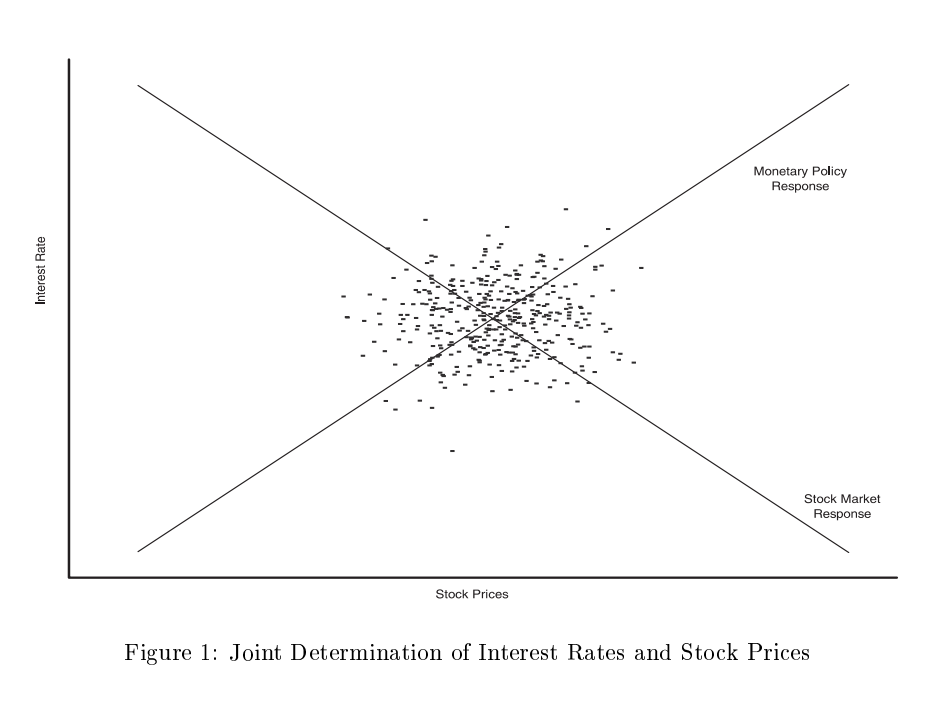
\includegraphics[width=\linewidth]{image/left Rigobon.png}
    \end{minipage}
    \hfill
    \begin{minipage}{0.48\linewidth}
        \centering
        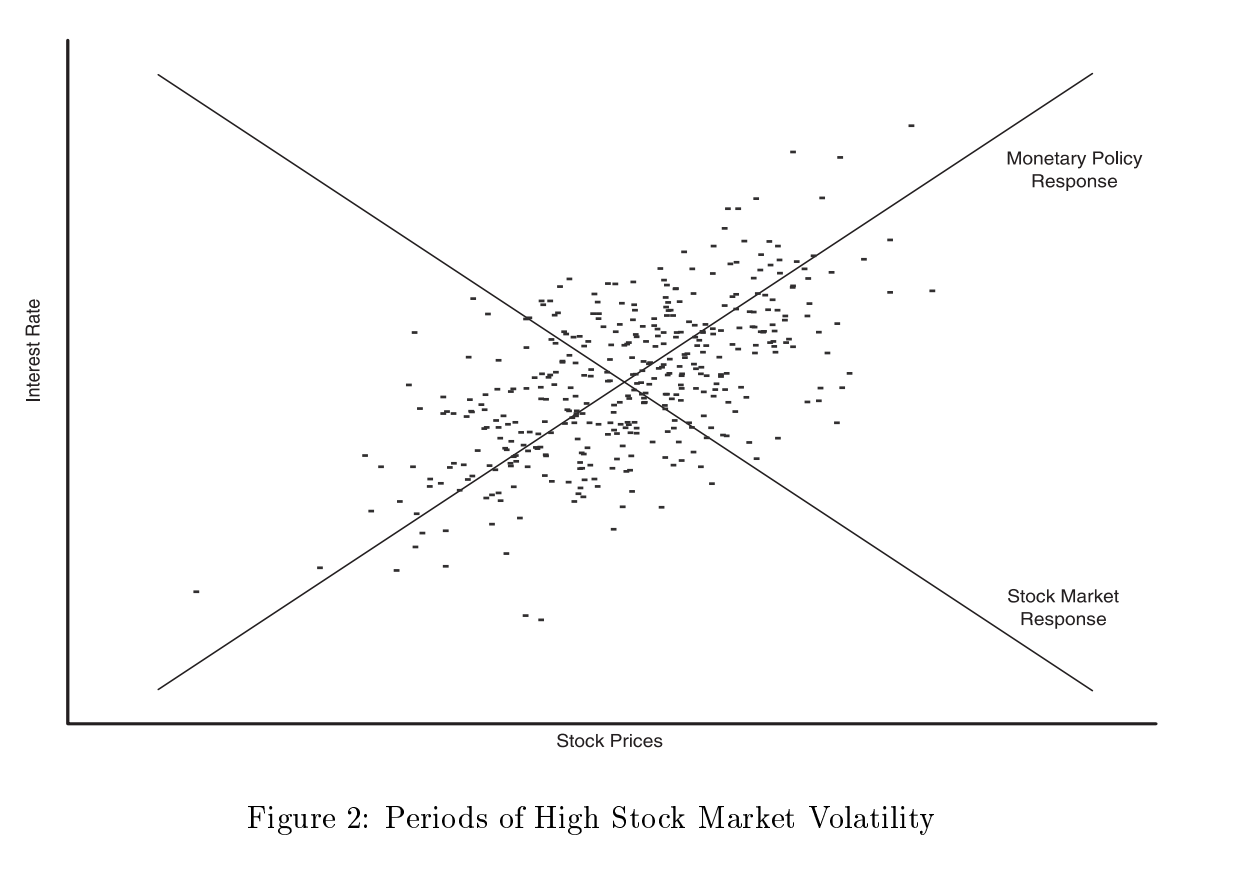
\includegraphics[width=\linewidth]{right ribodon.png}
    \end{minipage}
     \caption{\footnotesize The observed correlation between interest rates and stock prices reflects two simultaneous relationships. When stock-market shocks become more volatile, the data cloud stretches along the monetary-policy reaction function, allowing its slope to be identified from changes in the covariance matrix.}
    
\end{figure}
\end{frame}

\begin{frame}{What is assumed?}
\small

Identification is obtained because we assume:

\medskip

\begin{itemize}\itemsep5pt
  \item \textbf{Stable contemporaneous structure:} $B$ is the same across regimes.
  \item \textbf{Volatility shifts only:} what changes is $\Lambda_r$, not necessarily the propagation mechanism.
  \item \textbf{Again, orthogonal structural shocks:} $\Lambda_r$ is diagonal.
  \item \textbf{Different relative volatility changes:} otherwise shocks are only partially separated.
  \item \textbf{And regimes are \textit{meaningful}:} observed regimes or latent Markov regimes must capture real changes in volatility.
\end{itemize}

\medskip

Fragile if the crisis changes behaviours.

\end{frame}


\begin{frame}{Heteroskedasticity in practice}
\small

\textbf{How to use it empirically?}

\medskip

\begin{enumerate}\itemsep5pt
  \item Estimate a VAR, possibly allowing for volatility regimes.
  \item Estimate covariance matrices by regime.
  \item Recover structural directions using the joint diagonalisation logic.
  \item Label the shocks ex post using IRFs, variance shares, historical episodes, or additional weak restrictions.
\end{enumerate}

\medskip

\textbf{About \textit{meaningfulness}}, heteroskedasticity may \emph{identify directions} but not their economic names.

\end{frame}


\begin{frame}{Max share identification}
\small

Another idea: do not identify a shock by saying what it cannot do, but by saying what it \textbf{explains} \textbf{most}. E.g.,

\medskip

\begin{itemize}\itemsep5pt
  \item A technology shock can be defined as the shock explaining the largest share of productivity at a long but finite horizon.
  \item A news shock can be defined as the shock explaining a large share of future TFP with no contemporaneous TFP movement.
  \item A main business cycle shock can be defined as the shock explaining the largest share of GDP or aggregate volatility at business cycle frequencies.
\end{itemize}

\medskip

$\Longrightarrow$ operational definition of a shock as a \textbf{dominant driver} for a variable, horizon or frequency band.

\medskip

\footnotesize Francis, Owyang and Roush (2014); Barsky and Sims (2011); DiCecio and Owyang (2010); Angeletos, Collard and Dellas (2020).

\end{frame}


\begin{frame}{Finite horizon max share}
\small

\textbf{Idea:} among all orthogonal rotations, pick the shock that explains most of variable $j$ over horizons $0,\ldots,H$.

\medskip

For variable $j$ and horizon $H$, choose the following shock $q$:
\[
q^\star = \arg\max_{q'q=1}
\sum_{h=0}^{H}\left(e_j'\Phi_hPq\right)^2.
\]

\medskip

The denominator of the FEVD does not depend on $q$. Hence this is an eigenvector problem.



\end{frame}


\begin{frame}{Spectral max share}
\small

Instead of choosing a horizon $H$, choose a \textbf{frequency band}.

\medskip

Example: $\Omega_{BC}$ periodicities between 6 and 32 quarters.

\medskip

The \textbf{\textit{spectral density}} implied by the VAR tells us how much variance of $y_j$ lies at each frequency. A candidate shock $q$ explains part of that frequency specific variance.

\[
q^\star = \arg\max_{q'q=1}
\int_{\omega\in\Omega}
\left|e_j'\Phi(e^{-i\omega})Pq\right|^2 d\omega.
\]


Again an eigenvector problem, but now the objective is not ``explains variable $j$ after $H$ quarters'' but ``explains variable $j$ at the frequencies we call the cycle''.

\medskip
Angeletos, Collard and Dellas' \textit{Business Cycle Anatomy} (2020) identify a \textbf{Main Business Cycle shock} as the shock that captures the maximal share of macroeconomic volatility at business cycle frequencies. Then they ask: can DSGE mechanisms generate a shock with this propagation pattern?
\medskip

\textbf{Excellent for summarising a cycle.} 

\end{frame}


\begin{frame}{Spectral max share}

\centering

\begin{figure}
    \centering
    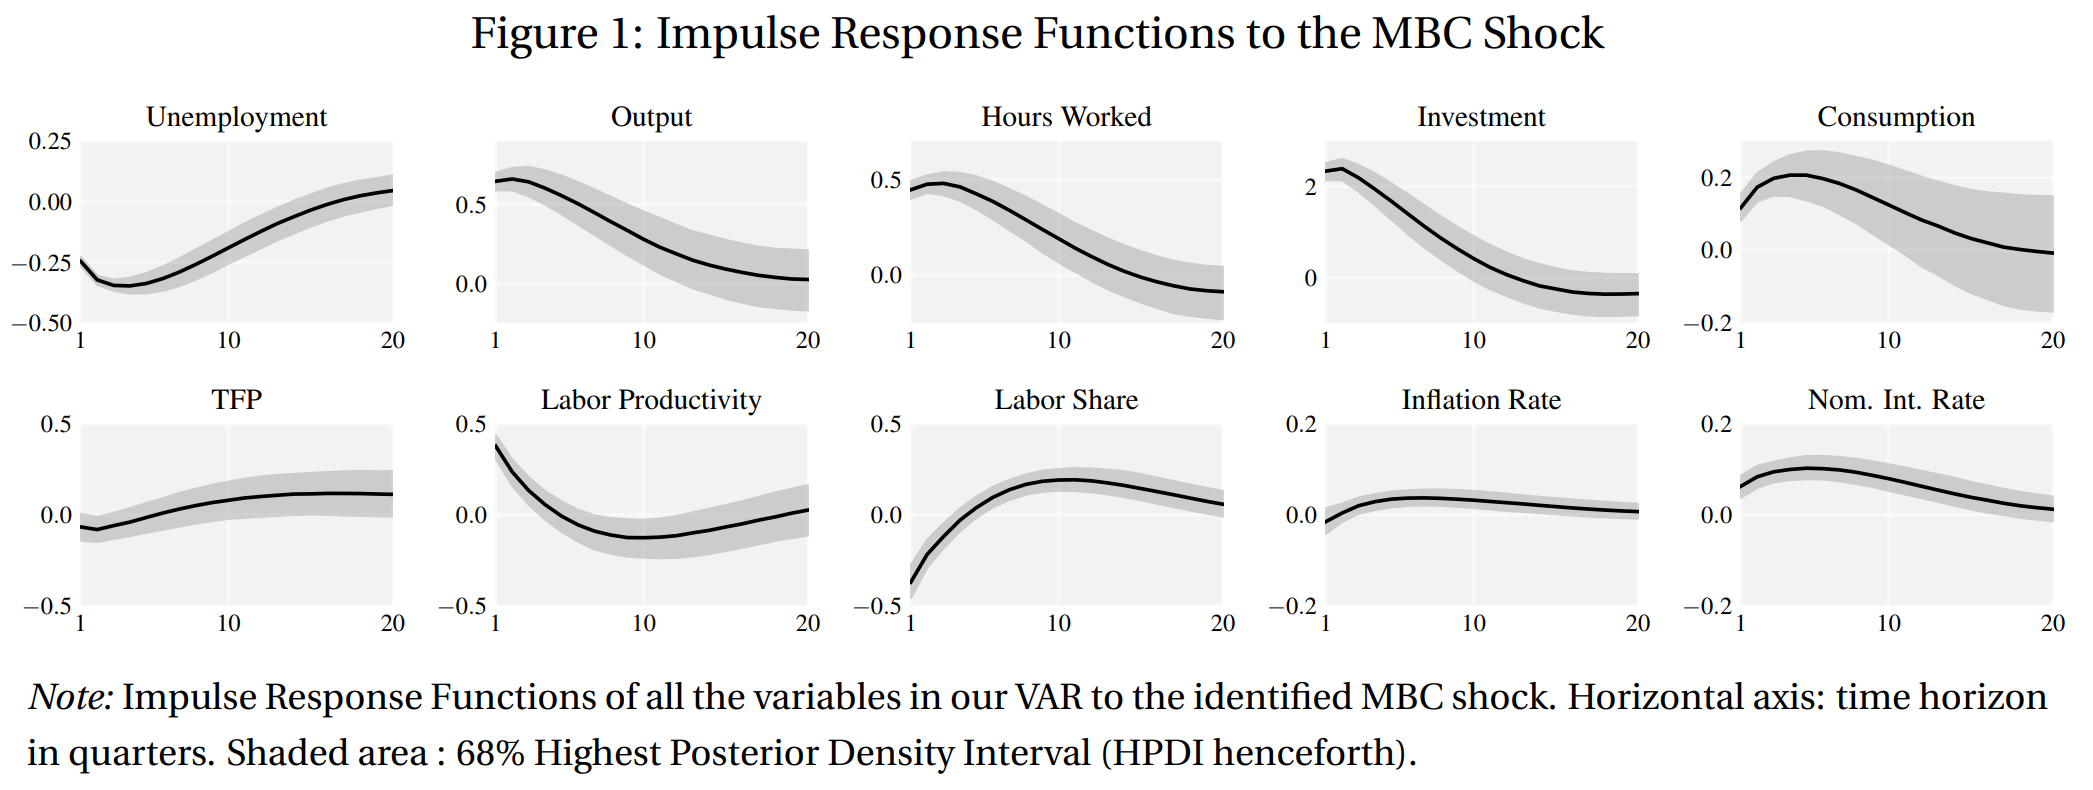
\includegraphics[width=1\linewidth]{image/MBC ACD.png}
    \caption{Angeletos et al. (2020)}
\end{figure}

\end{frame}




\begin{frame}{Max share: algorithm}
\footnotesize

\begin{enumerate}
  \item Estimate the reduced form VAR.
  \item Compute $\Phi_h$ or the frequency response $\Phi(e^{-i\omega})$.
  \item Choose the target: variable, set of variables, horizon, or frequency band.
  \item Build the positive semi definite matrix of explained variance.
  \item Take the leading eigenvector $q^\star$.
  \item Compute IRFs, FEVD, historical decomposition for $Pq^\star$.
\end{enumerate}


\textbf{Strengths:}
\begin{itemize}
  \item avoids very strong long run zero restrictions;
  \item works at finite horizons or frequencies;
  \item useful when the question is: what is the dominant driver of this object?
\end{itemize}

\textbf{Limits:}
\begin{itemize}
  \item the label of the shock is not delivered by the eigenvector;
  \item different targets can generate different shocks;
  \item a dominant statistical driver need not be a primitive structural cause;
  \item informational insufficiency can contaminate the recovered shock.
\end{itemize}


\end{frame}



\end{document}

